\documentclass{thesis}

\usepackage{pdfpages}

\begin{document}

% Metadata ====================================================================

\title{Regressing Litter on Deprivation in Glasgow City with Object Detection}
\author{Gary Blackwood}
\date{\today}
\maketitle

% Abstract ====================================================================

\begin{abstract}

This study explored the relationship between deprivation in Glasgow City and the amount of litter on its streets. It also aimed to discover if an automated approach to quantifying litter on a city-scale could be achieved using object detection methods. A YOLOv5s object detection model was developed and applied to detect litter in 37,300 Google street view images of locations all over Glasgow City. The detected litter was enumerated and made searchable by a publicly available \href{https://glasgow-litter.garyblackwood.co.uk}{web application} that allows users to interactively explore a map visualisation. The resulting counts were combined with deprivation indicators provided by the Scottish Index of Multiple Deprivation publication. A Negative Binomial count data regression model was developed to identify the relationships between deprivation and litter. The application of the object detection model produced a 77\% true positive rate over 254 littered objects, with only 28 false positives. This suggests that it may generalise well to unseen data. It was discovered that no deprivation indicators were statistically significant explanatory regression variables at a significance level of $\alpha = 0.05$, although a breakthrough may be possible by overcoming limitations such as data quantity, quality, and hardware resources. The findings indicate that there is no relationship between deprivation and the amount of litter in Glasgow City. However, there is uncertainty in this conclusion due to the limitations of the approach taken to quantify litter. By addressing the limitations present, it is acknowledged that there is great potential in using object detection to count litter at scale.

\end{abstract}

% Acknowledgements ============================================================

\chapter*{Acknowledgements}

I would like to express my sincere gratitude to my supervisor Dr Andrew Elliott for his invaluable advice and assistance throughout the project. I am also deeply grateful to my family for their unwavering support.

% List of Figures and List of Tables ==========================================

\listoffigures
\listoftables

%==============================================================================

\tableofcontents

% Introduction ================================================================

\chapter{Introduction}
\pagenumbering{arabic} % Don't remove this!

In 1982, Wilson \& Kelling popularised the theory that an urban environment with visible signs of disorder promotes even further disorder. Known as the "Broken Windows" theory, they suggested that normalising behaviour such as vandalism by leaving it unaddressed increased the likelihood that crime and civil disobedience would occur\cite{broken-windows}. If individuals use the general appearance of a neighbourhood as a sign of the expected social norms, then a disordered environment sends the message that lawlessness goes unpunished. An ordered environment on the other hand, in which the windows remain intact, bodes that bad behaviour will not be tolerated.

The discourse surrounding the theory shifted from praise to criticism as researchers scrutinised the claims. Nowadays, it is controversial to promote a causal link between disorder and crime as subsequent studies have found no evidence\cite{OBrien2019LookingTB}. In 2019, O’Brien et al. analysed 300 studies to reveal that disorder in a neighbourhood does not directly cause its residents to commit more crimes.

A physical sign of disorder that negatively impacts an area's presentation is the amount of visible litter on its streets. If the assumption holds that a neighbourhood's appearance can communicate with its inhabitants, to what extent does littering encourage disorderliness?

According to a recent study by Keep Scotland Beautiful, the issue of litter creates the most public outcry and is an important indicator of overall environmental quality\cite{household-survey-2019}. Unfortunately, the study found that since 2016, the state of our public spaces has been in decline. None more so than in the most deprived areas of the country where the number of significantly littered sites has more than doubled since 2014. Why is there more litter in the most deprived areas? The socioeconomic problems that come with deprivation may be the answer.

Littering behaviour is strongly affected by the social context in which it occurs\cite{littering-behaviour}. Research by Zero Waste Scotland found that in addition to personal factors such as age and gender, social factors influenced the prevalence of litter. If individuals in an area deem it socially acceptable, it is more likely to occur. 

The Scottish Government seeks to understand the circumstances surrounding deprived communities to make effective policy-making decisions. If there are links between deprivation and littering, there may be the potential for the improvement of one issue to improve the other. Tackling litter by creating a fairer society is an exciting thought, but first, we must discover the links between litter and deprivation.

This study aimed to identify the relationships between the key indicators of deprivation in areas of Glasgow City and the amount of litter on its streets. To this end, the Poisson and Negative Binomial regression models for count data were employed. The ambition was to discover areas of focus that could reduce littering if improved.

Secondary to this aspiration, it was of interest to discover if an automated approach to counting litter on a city-scale could be achieved using deep learning object detection methods. Thus far, local organisations have had to perform manual audits to collect such data. Any improvement to this process would be a welcome step towards a cleaner world.

Finally, an extensive software component was developed to increase the accessibility of the results. By allowing interested parties to explore the litter detected within Glasgow City, as well as run the detection themselves, the aim was to help inform the policy-making decisions of non-technical users.

% Literature Review ===========================================================

\chapter{Literature Review}

\section{Object Detection}

The purpose of an object detector is to take an input image and search it for a subset of object classes before surrounding those identified in a bounding box. Applications include the real-time detection of other vehicles in self-driving cars, and anomaly detection during manufacturing processes. Such detectors are useful when working with real-time video feeds, but can also detect using recorded images. 

\begin{figure}[h]
    \centering
    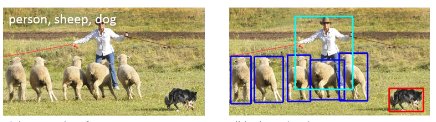
\includegraphics[scale=1]{images/person-sheep-dog.PNG}
    \caption{An example of image classification (left) and object localisation (right.) Images taken from \cite{lin2015microsoft}.}
    \label{fig:cnn-diagram}
\end{figure}

This section outlines two popular object detection models that were used throughout the study: You Only Look Once and Faster Region-based Convolutional Neural Network. We will describe how they use convolutional neural networks to detect objects and discuss how their performance is evaluated. Finally, we will cover existing attempts to detect litter using object detection. Further exploration of the methods will be covered in chapter \ref{chapter:methods}.

\subsection{Convolutional Neural Networks}

To recognise patterns and ultimately objects within an image, we can use convolutional neural networks to identify shapes such as lines, circles and gradients. Modelled after the human brain, they are composed of many layers of artificial neurons that can be thought of as mathematical functions that calculate the weighted sum of many inputs. When applied for object detection, a convolution converts all the pixels into a single value. The output of an entire convolutional layer is therefore a vector of such values. A layer of neurons produces an activation map which highlights features of the input. For example, a feature of an image input may be a vertical edge. They use activation functions that transform features as they flow through the network. Activation maps from one layer are provided as input to the next layer in order to extract even more complex features. Known as convolutional layers, they start detecting higher-level features, such as entire objects, the deeper you go. A final classification layer is responsible for producing the probabilities that the input belongs to a particular class based on the features provided by the last convolutional layer.

\begin{figure}[h]
    \centering
    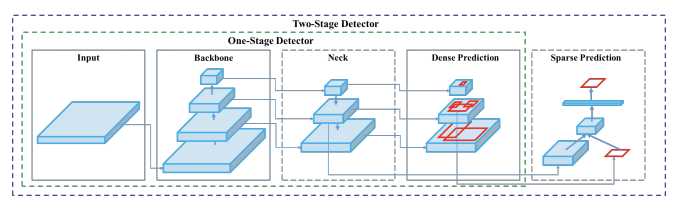
\includegraphics[scale=0.6]{images/cnn-diagram.png}
    \caption{The anatomy of an object detector. Diagram taken from \cite{yolov4}.}
    \label{fig:cnn-diagram}
\end{figure}

CNN object detectors use supervised learning and generally consist of two components; a CNN-based backbone that is used for feature extraction, and a head that is used to predict the class and bounding box for an object. In recent years, state-of-the-art models have begun to insert layers in-between the backbone and head to form a third component known as the neck.

The backbone component is the CNN responsible for computing features from an input image. The input to the first convolutional layer will be the pixels of that image. Existing Backbones are typically used for their proven feature extraction capabilities on classification problems. Rather than redesign custom networks, researchers will fine-tune the backbone to increase its suitability to the task at hand. Commonly used backbones include ResNet, VGG, and CSPDarknet53\cite{zhu2021tphyolov5}. These are typically pre-trained using the ImageNet\footnote{https://www.image-net.org} data set to adapt the weights to identify relevant image features\cite{breakdown-yolo4}.

The purpose of the neck is to improve upon the features provided by the backbone. Usually consisting of several bottom-up and top-down paths, the neck reprocesses the backbone's features at different stages with the goal of aggregating them in preparation for the detection in the head.

The responsibility of detecting the location and category of an object falls upon the head. It takes the features extracted from the preceding layer's classification network and turns them into a prediction. 

There are generally two kinds of object detectors: one-stage and two-stage. Two-stage detectors have separate phases for bounding box and class predictions and for many years this was the most popular method. The R-CNN series of detectors\cite{frcnn} is a representative example. One-stage detectors, like You Only Look Once (YOLO), accept the trade-off of faster detection for lower accuracy by performing bounding box and class prediction at the same time.

\subsection{Evaluation}

Evaluating object detection is challenging as it involves performing classification to determine whether or not an object exists, and localisation to determine the location of that object. 

A typical data set will contain a non-uniform distribution of many classes. If a simple accuracy based metric was used for evaluation a biased result would be produced. It is for this reason that the the mean average precision (mAP) metric is used.

The mean average precision (mAP) quantifies the performance of an object detector across all test images, classes, and at different confidence thresholds.

To calculate mAP and measure correctness, overlap between the predicted bounding box and ground truth box is measured using its intersection over union (IoU). 

\begin{equation}
    IoU = \frac{Area of Overlap}{Area of Union}
\end{equation}

Precision and recall measures are calculated for a class using the IoU value for many IoU thresholds. If the IoU value is greater than the threshold, the prediction is treated as a true positive. Otherwise, it is considered a false positive. The precision measures the percentage of correct predictions made and the recall measures the percentage of positives that were correctly identified. An object detector can trade-off precision for recall and vice-versa by adjusting the confidence threshold needed to make a prediction.

\begin{figure}[h]
    \centering
    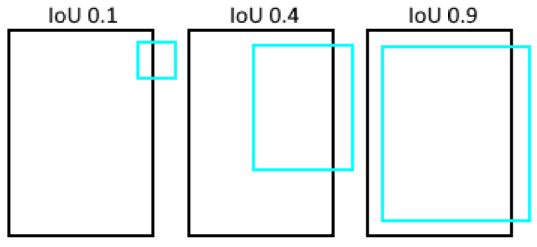
\includegraphics[scale=0.5]{images/iou.png}
    \caption{A minimal visualisation of intersection of union at different values.}
    \label{fig:cnn-diagram}
\end{figure}

Precision-recall curves are constructed by setting the IoU threshold at varying levels of difficulty e.g. from 0.5--0.95 in increments of 0.05. The average precision (AP) is calculated individually for each class, before finally being averaged across all classes to produce the evaluation metric.

As a complement to mAP, the F1 metric combines the precision and recall measures to find the ideal confidence threshold which maximises them both. Similarly,
the area under the curve (AUC) metric integrates the amount of plot that falls underneath the precision-recall curve.

Most state-of-art object detectors publish their results using the mAP evaluation of well known challenges such as COCO\cite{lin2015microsoft} and Pascal VOC\cite{Everingham15}. However, as it depends on a subjective confidence level there can be a large gap between it and the actual accuracy\cite{Peng2021}. Researchers have studied ways to address this for classification problems by calibrating the confidence level beforehand\cite{guo2017calibration}, but material for object detection is minimal due to its complexity.


\subsection{YOLO}

You Only Look Once (YOLOv1), a neural network-based approach to object detection, was first published in a 2015 paper titled \textit{You Only Look Once: Unified, Real-Time Object Detection}. The paper describes how the authors combined a previously multi-step object detection process into a single neural network that performs classification and bounding box detection.

The motivation of the authors was for the detector to literally "only look once", such that a single neural network would produce vectors of object predictions when given an input image.

With a unified structure facilitating end-to-end optimisations on detection performance, the network can outperform existing methods such as R-CNN in terms of accuracy and speed\cite{yolov1}. In contrast to detection systems that re-purpose classifiers, YOLO re-frames the task into a regression problem that outputs class probabilities and bounding boxes by inspecting each image only a single time. 

The researchers found that training on full images brought about several benefits. With the ability to view the entire image, the model includes contextual information that competing methods are missing\cite{frcnn}. The result is a model that makes less than half the number of background errors compared to Fast R-CNN\cite{yolov1}.

As a result of its simplicity, the model is extremely fast because it only has to run its singular convolutional neural network on new images. With speeds up to 150 frames per second\cite{yolov1}, the model is promising for real-time applications.

It was found that the model performed well when applied to new domains because of its ability to learn generalisable representations of the objects it is detecting. However, it did not match the best performing detectors in terms of accuracy due to its difficulty in identifying the precise location of small objects.

In the follow-up paper, \textit{YOLO9000: Better, Faster, Stronger}, an improved version of the model is described. Known as YOLOv2, it addresses a number of its predecessor's shortcomings. The model's poor recall and aforementioned localisation errors are improved by modifications including the introduction of batch normalisation and increasing the resolution of the classifier\cite{yolo2}.

\textit{YOLOv3: An Incremental Improvement} presents further advancements that produced a bigger, but more accurate network. The paper highlights that although previous iterations of the model struggled with small objects, the third version reverses this trend. The trade-off, however, was the slightly worse performance on objects of medium and large size\cite{yolo3}.

The penultimate iteration of the model (YOLOv4) achieves state-of-the-art results by combining universal detection features that have little to no impact on training or inference time\cite{yolov4}. Mish-activation was added as an activation function that pushes its input to the left and right to achieve its optimal point. Cross mini-Batch Normalisation was added to make the network more stable by changing layer values to a common scale without requiring multiple GPUs. DropBlock regularisation was added to hide sections of an image from the first layer to force the network to learn features that it cannot rely upon to be visible.

\begin{figure}[h]
    \centering
    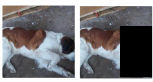
\includegraphics[scale=1]{images/dropblock.png}
    \caption{A dog's head hidden by DropBlock regularisation. Image taken from \cite{cutmix}.}
    \label{fig:dropblock}
\end{figure}


The publication highlights how the majority of accurate detectors do not facilitate real-time operation before explaining how this problem is overcome by creating a convolutional neural network for which training requires only a single conventional graphics processing unit with 8--16 GB of memory. The result is a model which is faster, in terms of frames per second, and more accurate, using the MS COCO AP metric, than all competition.

YOLOv5 is the latest object detector of its kind and it offers different pre-trained models including YOLOv5n, YOLOv5s, YOLOv5m, YOLOv5l and YOLOv5x. From smallest and fastest to largest and slowest respectively, each has a domain in which it is most appropriate. For example, the small YOLOv5s model can be deployed on mobile devices as it has significantly fewer parameters (millions) and requires considerably less GPU memory to train and run than the larger models\cite{yolov5}.

The architecture consists of a CSPDarknet53 backbone with a Spatial Pyramid Pooling layer that removes the fixed-size constraint of the network, and a PANet neck that is followed by a YOLO detection head\cite{yolov1}. The inner workings of these components are out of scope but for reference see \cite{yolov5}, \cite{cspnet}, \cite{spp}, and \cite{panet}. Modifications that did not increase, or only minimally increased the computational cost, are implemented as optimisations to improve accuracy\cite{yolov4}.

\subsection{Faster R-CNN}

One of the very first successful applications of convolutional neural networks to the problem of object detection resulted in the creation of a method known as R-CNN: Regions with CNN features\cite{rcnn}. This method first generates 2000 region proposals, which are subsets of the image highly likely to contain an object, before running each independently through a CNN to extract features that are classified by a class-specific support vector machine. This approach achieved leading detection performance on the Pascal VOC challenge data set with a mAP of 53.7\%.

\begin{figure}[h]
    \centering
    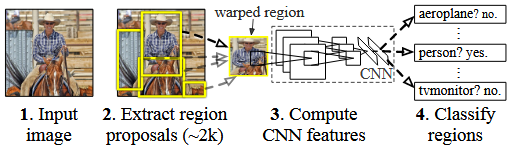
\includegraphics[scale=0.75]{images/rcnn.png}
    \caption{R-CNN object detection system overview. Diagram taken from \cite{rcnn}.}
    \label{fig:faster-rcnn-architecture}
\end{figure}

In a follow up to his original paper, the author proposed Fast R-CNN as a method that fixed the disadvantages of R-CNN while simultaneously improving its accuracy and speed\cite{fast-rcnn}. Building from this, the Faster R-CNN method made further improvements to reduce the proposal generation computational complexity. By sharing the same convolutional layers for the detector and Region Proposal Networks (RPN), the method was able to support passing an image through the network only once\cite{frcnn}.

\begin{figure}[h]
    \centering
    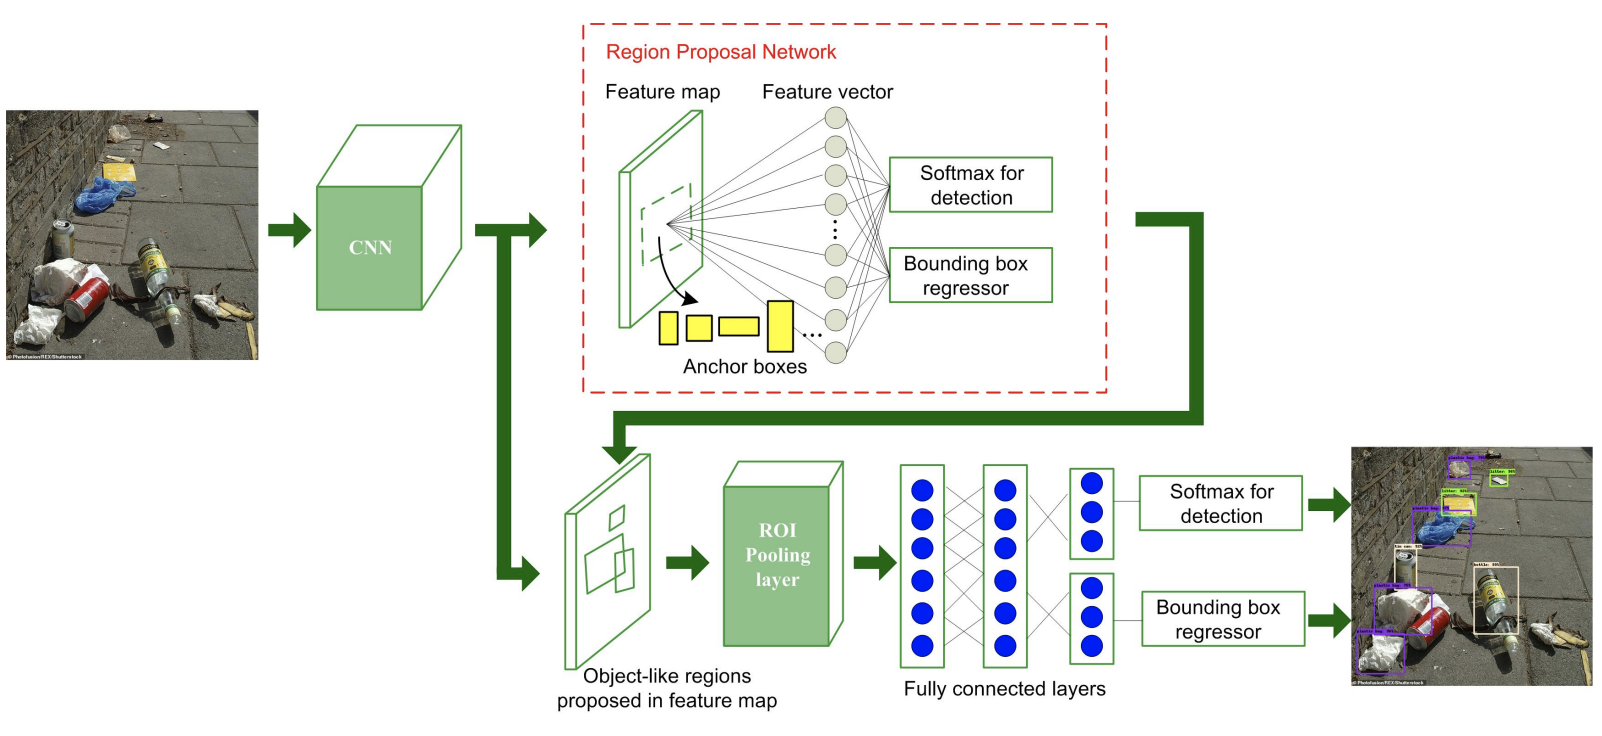
\includegraphics[scale=0.5]{images/faster-rcnn-architecture.png}
    \caption{The architecture of Faster R-CNN. Diagram taken from \cite{smart-street}.}
    \label{fig:faster-rcnn-architecture}
\end{figure}

Figure \ref{fig:faster-rcnn-architecture} illustrates how Faster R-CNN uses layers known as Region Proposal Networks to generate feature maps which are turned into object region proposals. The proposals are projected onto the feature map and objects are detected by classifying the proposals. Now a one-stage detector with a single network, Faster R-CNN, like YOLO\cite{yolov1}, can be trained end-to-end and optimised for detection performance.

\subsection{Litter Detection}

Attempts to quantify litter using automated object detection have been made\cite{cvstreets}. However, the lack of available data forced the researchers to manually collect and annotate images. In the paper, the researchers used a neural network-based model called OverFeat-GoogLeNe to reach 63.2\% of precision while having 61.02\% of recall for a cigarette butts class. A camera was attached to a vehicle and placed at a height of two to three meters from the ground. This limited the litter detection to objects within the immediate vicinity of the vehicle. It was highlighted that no prior work has been undertaken to develop such an automated approach.

The present paper aims to improve upon two aforementioned drawbacks: the images shall be automatically collected, and they shall show locations much further away from the location at which the image was taken. Furthermore, YOLO and Faster R-CNN object detection models shall be harnessed which should offer improved performance as they use more modern techniques.

Despite the availability of large data sets such as COCO\cite{lin2015microsoft}, litter is underrepresented due to its geographic and material variation. The Trash Annotations In Context (TACO) initiative aims to tackle this problem to improve autonomous litter monitoring systems\cite{DBLP:journals/corr/abs-2003-06975}. In its paper, the TACO researchers describe how it can often be impossible to distinguish between different types of litter due to the small size of the objects and the resolution of the images. Cigarettes, one of the most commonly littered objects, mostly covered an area less than 64x64 pixels in size. This issue compounds with the lack of available data, which they attempt to address using augmentation and transplantation techniques. A Mask R-CNN model was trained, but the lack of annotated images and difficulty detecting small objects significantly impacted the resulting AP performance. An AP of 26.2 was achieved for 4-fold cross-validation when detecting and segmenting litter. This dropped to 18.4 when classification to distinguish between ten types of litter was introduced. To this end they performed image augmentation by adding Gaussian blur and AWG noise, changing image
exposure and contrast, and rotating by 45 degrees. We will also only focus on detecting litter without caring about its class, and we will use a new mosaic augment that will be described in chapter \ref{chapter:methods}.

A Clean Europe Network summit meeting\footnote{https://cleaneuropenetwork.eu/en/measuring-litter/aus} concluded that a lack of data is contributing to the difficulty in addressing the environmental issues caused by urban littering. Cities throughout the world are assessing urban cleanliness by means of human audits. Without a practical approach to measuring an index of cleanliness, it will be challenging to properly manage the problem. 

Researchers in Spain proposed a cleanliness index for the city of Granada\cite{sevilla}. As part of its definition litter was weighted based on its classification, with larger objects assigned higher weights. The study used data that was manually collected by humans and provided by the organisation responsible for cleaning the city.

Efforts have also been made to automate the data collection process. Researchers in India have used the Microsoft Bing Image Search API to gather a large and diverse set of 2561 images that could be used to train a CNN for detecting litter\cite{Mittal2016SpotGarbageSA}. They provide an Android mobile application that can be used by citizens to report litter in their communities. The approach focused on segmenting areas of images taken by mobile phones, rather than the quantification of the litter itself. In their paper, the authors describe how they utilised a pre-trained AlexNet\cite{NIPS2012_c399862d} model to obtain a 90.06\% specificity and 83.96\% sensitivity.

\section{Regression}

The strength of a relationship between a dependent and independent variable can be assessed using regression analysis. In this case, our dependent variable is litter and the independent variables are the indicators of deprivation. We can use count data regression to understand which indicators influence the amount of litter present.

The inference of count data involves estimating the unknown parameters of a given probability distribution. The distribution models the number of occurrences of an event, such as train accidents in a given year, or a rate, such as the quantity of litter in a given area.

\subsection{Poisson}

The benchmark parametric model for count data is the Poisson distribution\cite{cameron_trivedi_2013}. It helps to predict the probability of an event occurring when you know how often it has already occurred. Shown in equation \ref{eq:poisson-model}, the model assumes that the response $Y$ follows the Poisson distribution and it is concerned with modelling the effects of explanatory variables on the response through the rate parameter $\mu$. 

\begin{equation}
    E(Y_i) = \mu_i = n_i\theta_i = n_ie^{x_i^t\beta},\hspace{1em}Y_i = Poi(\mu_i)
    \label{eq:poisson-model}
\end{equation}

The unknown rate parameter $\mu$ is defined in terms of units of exposure, which is the length of time during which the events are recorded\cite{cameron_trivedi_2013}. The parameter is the expected number of event occurrences.

\begin{figure}[h]
    \centering
    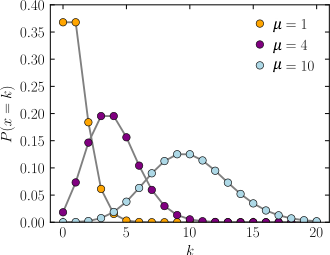
\includegraphics[scale=0.8]{images/poisson-pmf.png}
    \caption{The Poisson probability mass function showing the probability of $k$ occurrences given the expected rate $\mu$. Plot taken from \cite{poisson-wikipedia}.}
    \label{fig:poisson-pmf}
\end{figure}

Dependence on the explanatory variables is given by $\theta_i = n_ie^{x_i^t\beta}$ in which the $i$th covariate pattern is explained for exposure $n_i$. The corresponding link function with offset $\log{n_i}$ is given by:

\begin{equation}
    \log{\mu_i} = \log{n_i} + x_i^t\beta
\end{equation}

The mean and variance of $Y \sim Poi(\mu)$ are both $\mu$ and the probability mass function for the distribution is given in equation \ref{eq:possion-pmf}. 

\begin{equation}
f(y) = \frac{\mu^ye^{-\mu}}{y!},\hspace{1em}y = 0, 1, 2,...
\label{eq:possion-pmf}
\end{equation}

This equality of mean and variance is known as the \textit{equidispersion} property of the Poisson and it is frequently not the case for real-world data. \textit{Overdispersion} is said to occur if the mean exceeds the variance. Similarly, \textit{underdispersion} presents itself if the variance is less than the mean. When data exhibit this property, it needs to be accounted for so that statistical inferences are valid\cite{understanding-poisson}.

Poisson regression models have been applied in many domains including health, finance and manufacturing. In 1992, the number of defects per area in a manufacturing process at the AT\&T Bell Laboratories was studied\cite{defects}. The researchers used the zero-inflated variant of the model to identify the set of conditions under which the mean number of defects was lowest. The standard Poisson regression model was used in this study.

\subsection{Negative Binomial}

Violations of the equidispersion property of the Poisson regression model can be dealt with by assuming a negative binomial distribution for the response $Y$, which allows for variances that are not equal to the mean.

The model form is the same as the Poisson and it introduces a new unknown variable $\alpha$ with density:

\begin{equation}
    f(y|\mu,\alpha) = \frac{\Gamma(y + \alpha^{-1})}{\Gamma(y+1)\Gamma(\alpha^{-1})}(\frac{\alpha^{-1}}{\alpha^{-1} + \mu})^{\alpha^{-1}}(\frac{\mu}{\alpha^{-1} + \mu})^y,\hspace{1em}\alpha\ge 0, y=0,1,2,...
\end{equation}

Both $\mu$ and $\alpha$ are estimated during model fitting. It has been suggested that $\alpha$ should be chosen such that the Pearson or deviance static is equal to $n - k$\cite{cameron_trivedi_2013}.

The model reduces to the Poisson if $\alpha = 0$ as it is used to explain the variance which is $Var(Y_i) = \mu_i + \alpha\mu_i^2$ for the NB2 model: the most common implementation of the negative binomial\cite{cameron_trivedi_2013}. This formulation is popular because it allows the modelling of Poisson heterogeneity using a gamma distribution\cite{ncss-neg-bin}.

% Data ========================================================================

\chapter{Data} \label{chapter:data}

The data for the study were collected from three independent sources: The Scottish Government, Google, and Glasgow City Council. Python software programs were developed and run to obtain, prepare, and merge the data for object detection and regression analysis. This chapter describes the characteristics of the data, how many of them there are, where they have come from, and what they are used for.

\section{Scottish Index of Multiple Deprivation}

The Scottish Index of Multiple Deprivation (SIMD) is a tool for identifying the places in Scotland where people are experiencing disadvantages across different aspects of their lives \cite{simd}. Published by the Scottish Government, it provides a relative measure of deprivation across many small areas of the country.

The data are a collection of 6,976 data zones which represent areas with roughly equal populations of 700 -- 800 people (Figure \ref{fig:dz-total-populations}.) Each data zone has over 30 deprivation indicators such as crime rate, unemployment rate, and pupil attainment. See the table \ref{table:simd-deprivation-indicators} for a description of the indicators\footnote{For standardised ratios, a value of 100 is the Scotland average for a population with the same age and sex profile.}. By combining these indicators into a single index, the data zones are ranked relative to one another, from 1 -- 6,976, where rank 1 is the most deprived area in the country. In total, seven aspects of deprivation are combined: income, employment, health, education, skills and training, geographic access to services, crime, and housing. The weighted sum of these seven domains is taken to produce the overall SIMD\footnote{The weightings are outlined in the technical notes\cite{simd-technical-notes}.}.

\begin{figure}[h]
    \centering
    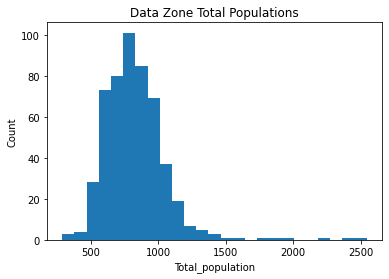
\includegraphics[scale=0.6]{images/dz-total-population.png}
    \caption{The total populations of Glasgow City's 746 data zones.}
    \label{fig:dz-total-populations}
\end{figure}

For the purposes of the study, the subset of data zones located in the Glasgow City council area was obtained, resulting in a collection of 746 data zones. Figure \ref{fig:glasgow-uni-dz} is one such data zone.

A revised version of the January 2020 publication was used for the study, in which the income domain and overall rankings were updated as a result of an error in the original data provided by the Department for Work and Pensions\footnote{https://www.gov.scot/publications/scottish-index-of-multiple-deprivation-2020v2-revision-notice}.

\begin{table}[ht!]
    \centering
    \begin{tabular}{||l p{100mm}||} 
     \hline
     \textbf{Indicator} & \textbf{Description} \\ [0.5ex] 
     \hline\hline
     Data\_Zone & Data zone name (string) \\
     Intermediate\_Zone & Intermediate zone name (string) \\
     Council\_area & Council area name (string)  \\
     Total\_population & Area population estimate (integer) \\
     Working\_age\_population & Area working age population estimate using state pension age (integer) \\
     income\_rate & Percentage of people who are income deprived \\
     employment\_rate & Percentage of people who are employment deprived \\
     employment\_count & Number of people who are employment deprived (integer) \\
     CIF & Comparative illness factor (standardised ratio) \\
     ALCOHOL & Hospital stays related to alcohol use (standardised ratio) \\
     DRUG & Hospital stays related to drug use (standardised ratio) \\
     SMR & Standardised mortality ratio (standardised ratio) \\
     DEPRESS & Percentage of population being prescribed drugs for anxiety, depression or psychosis \\
     LBWT & Percentage of live singleton births of low birth weight \\
     EMERG & Emergency stays in hospital (standardised ratio) \\
     Attendance & Percentage of school pupil attendance \\
     Attainment & Attainment score of school leavers (float) \\
     no\_qualifications & Working age of people with no qualifications (standardised ratio) \\
     not\_participating & Percentage of people aged 16 -- 19 not participating in education, employment or training \\
     University & Percentage of 17 -- 21 year olds entering university \\
     drive\_petrol & Average drive time to a petrol station in minutes (float) \\
     drive\_GP & Average drive time to a GP surgery in minutes (float) \\
     drive\_PO & Average drive time to a post office in minutes (float) \\
     drive\_primary & Average drive time to a primary school in minutes (float) \\
     drive\_retail & Average drive time to a retail centre in minutes (float) \\
     drive\_secondary & Average drive time to a secondary school in minutes (float) \\
     PT\_GP & Public transport travel time to a GP surgery in minutes (float) \\
     PT\_Post & Public transport travel time to a post office in minutes (float) \\
     PT\_retail & Public transport travel time to a retail centre in minutes (float) \\
     broadband & Percentage of premises without access to super fast broadband (float) \\
     crime\_count & Number of recorded crimes of violence, sexual offences, domestic housebreaking, vandalism, drugs offences, and common assault (integer) \\
     crime\_rate & Number of recorded crimes of violence, sexual offences, domestic housebreaking, vandalism, drugs offences, and common assault per 10,000 people (integer) \\
     overcrowded\_count & Number of people in households that are overcrowded (integer) \\
     nocentralheat\_count & Number of people in households without central heating (integer) \\
     overcrowded\_rate & Percentage of people in households that are overcrowded \\
     nocentralheat\_rate & Percentage of people in households without central heating \\ [1ex] 
     \hline
    \end{tabular}
    \hspace{100mm}
    \caption{A description of the SIMD data zone deprivation indicators.}
    \label{table:simd-deprivation-indicators}
\end{table}

\begin{figure}[h]
    \centering
    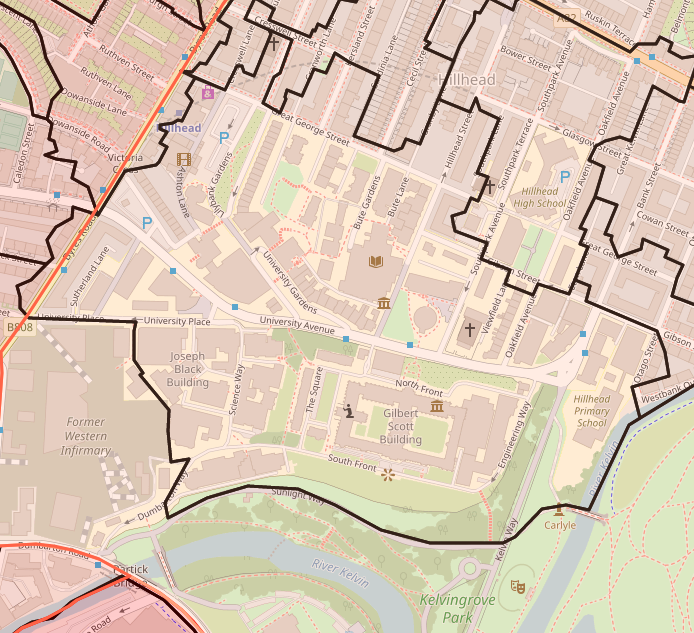
\includegraphics[scale=0.5]{images/glasgow-uni-ward.PNG}
    \caption{The data zone containing the University of Glasgow (S01010379). Mapping from \href{https://www.openstreetmap.org}{Open Street Map}.}
    \label{fig:glasgow-uni-dz}
\end{figure}

\subsection*{Missing Data}

A total of 137 missing indicator values were discovered in the data for Glasgow City. Indicated by a $*$ character, the missing value is used when a value cannot be determined, or if the value has been suppressed for disclosure control where small numbers are involved. The missing values were not concentrated in certain data zones but were prevalent in the \textit{Attendance} and \textit{Attainment} indicators. 

To maintain as much information as possible in the small data set, missing values were imputed as the mean of the observed values. The results are not particularly sensitive to the missing values as there are relatively few of them.

\subsection*{Litter Response}

To answer the questions of interest, the amount of litter in each Glasgow City data zone was quantified and added to the SIMD data set as integer counts. The object detection methods used to achieve the creation of this response variable are described in chapter \ref{chapter:methods}.

\section{Google Street View Images}

To achieve quantification of litter using object detection, thousands of images depicting the streets of Glasgow City were downloaded from the Google Maps Platform to be used as input to the object detection models. 

Software\footnote{https://github.com/Garee/glasgow-litter/scripts} was developed to obtain the images using the Street View Static API\footnote{https://developers.google.com/maps/documentation/streetview/overview}. Using a Python script, a uniformly random sample of 50 unique locations was generated within each data zone boundary and an image was downloaded at each. Object detection was later performed on these images to count the number of littered objects detected within each data zone. Another Python script counted the instances and combined the counts with the SIMD data set as the response variable. 

A total of 37,300 images (50 for each data zone) were retrieved at the maximum resolution of 640x640 pixels at a pitch of 0 degrees with a 90-degree field of view from the source camera on the vehicle. The pitch and field of view were chosen to obtain images of what was immediately beside the car as it travelled along the road. This view is ideal for being able to see roadside litter while also showing what is further away from the road. The images returned by Google have human faces and vehicle license plates automatically blurred to protect the privacy of individuals.

\begin{figure}[h]
    \centering
    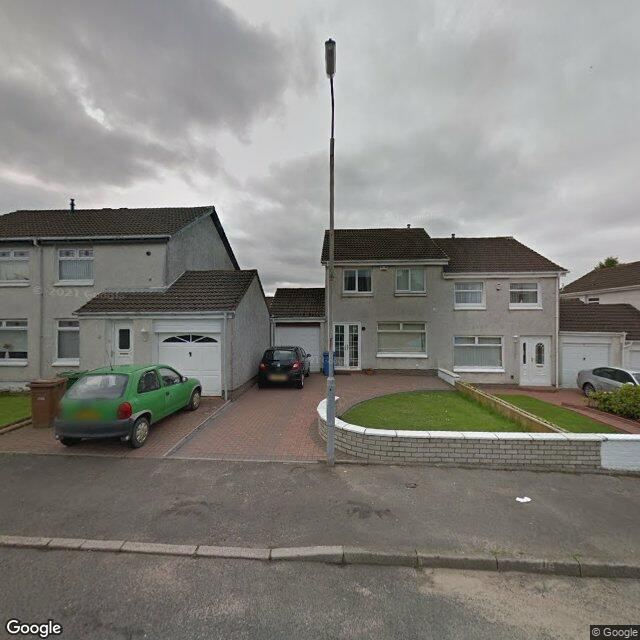
\includegraphics[scale=0.4]{images/street-view-image.jpg}
    \caption{A typical image of a Glasgow City street retrieved using the Google Maps Platform.}
    \label{fig:street-view-image}
\end{figure}

\section{Public Recycling Facility Locations}

The location and details of Glasgow City's 741 public recycling facilities were requested in JSON format from the public map that is hosted and maintained by Glasgow City Council.

Software was developed to count the number of facilities within each data zone boundary and add them to the SIMD data set as integers such that the count could be used as a potential explanatory variable.

Figure \ref{fig:public-recycling-points-analysis} shows that roughly half of all data zones have no public recycling facilities at all. Those that do typically have between one and four, while a few outliers have up to 11. During later analysis, it was discovered that there did not appear to be a correlation between the number of public recycling facilities and the amount of litter present in a data zone as Pearson's coefficient was 0.013.

\begin{figure}[h!]
    \centering
    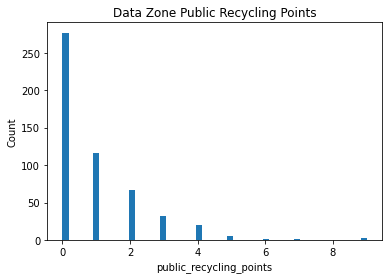
\includegraphics[scale=0.6]{images/data-zone-public-recycling-points.png}
    \caption{The number of public recycling facilities in each data zone.}
    \label{fig:public-recycling-points-analysis}
\end{figure}



% Methods =====================================================================

\chapter{Methods} \label{chapter:methods}

\section{Litter Detection}

To quantify the amount of litter in a data zone, the computer vision technique of object detection was performed to identify litter in the street view images that were chosen uniformly at random from within that data zone. This technique localises any litter in an image and assigns it a litter target class. To this end, the technique took as input a single street view image and produced zero or more $[x_1,y_1,x_2,y_2$] bounding box coordinates that determined the location of the litter within that image. Non-max suppression is used to select a single bounding box when many overlap using the intersection over union (IoU) evaluation metric. This task was repeated fifty times for each data zone before summing the number of bounding boxes to produce an overall count of litter. The location of the litter within the image was not of interest for the objectives of this study.

\subsection{Data Preparation}

\subsubsection{Data Labelling}

7,260 street view images of Glasgow City were hand-annotated to produce a collection of labelled images that could be used to train the object detection models. The images were selected uniformly at random from within the Glasgow City boundary. Upon completion, it was found that only a subset of 1,219 images contained litter; roughly one out of every six. The open-source data labelling tool Label Studio\footnote{https://labelstud.io} was used for this process.

As litter are generally small objects, and as the images were limited to a resolution of 640x640 pixels, it was often impossible to determine the type of litter that was being annotated. For this reason, only a single target class of \textit{litter} was used. Fortunately, this was enough for the goal of quantification. It also avoided the issue of an imbalanced label distribution, in which some classes are significantly more frequent than others.

To maximise the performance of the resulting models it was important to annotate consistently and with consideration. As I was the only individual labelling, the potential variability introduced by the subjectivity of multiple participants was not a worry. A tight box was annotated around the litter, and deposits of multiple littered objects were annotated individually.

\subsubsection{Data Split}

The images were split into training, validation and test data sets uniformly at random using an allocation of 70\%, 20\%, and 10\% respectively. The motivation was to prevent model overfitting in which it hyper-specifies to the training data, and does not generalise well to never before seen images. When this occurs, the loss function that determines how close the model is to making an accurate prediction ever decreases for the training data set, but eventually increases for the held-out validation data set. There is the possibility that validation loss may increase before decreasing again, in a scenario known as double-dipping. However, this was not observed during model development. The model was trained using the training data, selected using the validation data, and finally evaluated using the test data.

The split was taken from the disproportionately stratified sample of 1,219 images containing litter. This was to avoid under-representing the stratum of images containing litter, as most of the 7,260 images do not have any present. As the subsequent regression analysis results depend heavily upon the accuracy of the object detection model, it was important to provide sufficient enough images containing litter to learn from. A consequence of this decision will be to bias the model towards predicting false positives in images that do not contain any litter.

As the validation data set was used heavily during model creation and influenced the chosen model, a separate independent test data set was also held back. This was used to produce evaluation metrics at the end of the study to gauge a sense of how well the final model performs.

To avoid a train-test bleed in which the test data set is overly similar to the training data set, a Python script was developed and run to verify that there were no duplicate images.

\subsubsection{Data Preprocessing}

Null filter and contrast preprocessing steps were applied to all three data set splits to standardise them\footnote{Image transformations were performed using the online service Roboflow.}. Resizing was not necessary as all images were collected at a resolution of 640x640 pixels. 

To train our model to know that a street view may exist without litter, which is often the case, it was important to include null labelled images in the training data set. This is an important step to reduce false positives. To achieve this, a null filter was applied that guaranteed that at least 80\% of the training data contained labelled litter, while still allowing for those with none. The null labelled images were generated during mosaic augmentation as described in the next subsection.

A contrast preprocessing step was applied to exaggerate the differences between neighbouring pixels to improve edge detection\cite{roboflow-contrast}. This is helpful as google street view images are not all alike; they are taken at different times of day and in different weather conditions. By adjusting the contrast using adaptive equalisation to smooth the contrast, the resulting model may be more accurate.

\begin{figure}[h!]
    \centering
    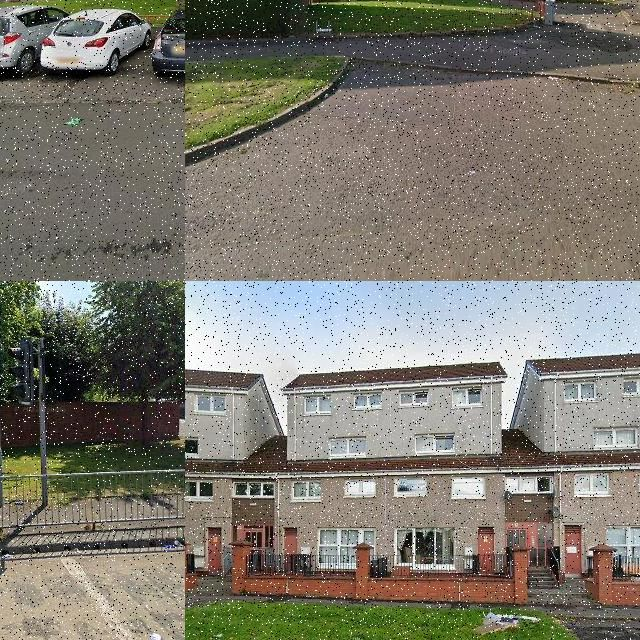
\includegraphics[scale=0.4]{images/mosaic-noise-example.jpg}
    \caption{An example of an augmented training image using the mosaic and noise techniques.}
    \label{fig:mosaic-noise-image}
\end{figure}

\subsubsection{Data Augmentation}

Image augmentations were applied to increase the size of the training set. These made slight alterations to the collected training data to produce new images, and therefore more information, for the model to learn from. This was an efficient way to generate thousands more training images without having to perform additional time consuming manual labelling. The test images were not augmented, as these were used during evaluation procedures.

The mosaic augmentation combined four source images into one by simulating four random crops while maintaining the relative scale of the litter. It aims to improve performance in terms of translation, and it also varies the amount of litter present in the images. This is because a mosaic image can potentially include litter from multiple other image sources. This was an important augmentation as it greatly increased the number of available training images.

Uniformly sampled noise replaced a maximum of up to 5\% of pixels for any given training image. This aimed to reduce over-fitting by applying variation to the data such that the model can better handle the imperfections that can be encountered in street view images.

\begin{table}[ht!]
    \centering
    \begin{tabular}{|l| |c|} 
     \hline
      \textbf{Augmentations} & \textbf{\# Training Images} \\
     \hline\hline
     None & 853 \\
     Mosaic x2 & 1,706  \\
     Mosaic x2, Auto-adjust Contrast & 1,706  \\
     Mosaic x3 & 2,559\\
     Mosaic x3, 5\% Noise & 2,559 \\
     Mosaic x3, Auto-adjust Contrast, 5\% Noise & 2,559 \\
     \hline
    \end{tabular}
    \hspace{100mm}
    \caption{The image augmentations and resulting non-cumulative training set sizes used for each trained model.}
    \label{table:model-augmentations}
\end{table}

\subsection{Hardware}

All object detection models were created using a personal computer to minimise compute costs. The time taken to train a single object detection model on the training data was typically in the region of 2 -- 5 hours, depending on the chosen number of epochs. Table \ref{table:hardware} describes the specifications of the key components that would impact total training time.

\begin{table}[ht!]
    \centering
    \begin{tabular}{|c| |c|} 
     \hline
     \textbf{Component} & \textbf{Description} \\ [0.5ex] 
     \hline\hline
     CPU & AMD Ryzen 5 5600X \\
     GPU & NVIDIA RTX 3060 12GB \\
     RAM & 32GB 3200Mhz Dual Channel  \\
     \hline
    \end{tabular}
    \hspace{100mm}
    \caption{The key hardware specifications used during model creation.}
    \label{table:hardware}
\end{table}

\subsection{YOLO}

Multiple YOLOv5 object detection models were trained and evaluated. This involved iteratively, in batches, improving the way the models mapped images to predictions. Techniques such as transfer learning, hyper-parameter tuning, and the aforementioned images augmentations were performed in an attempt to produce the best training results possible.

\subsubsection{Transfer Learning}

To start from a strong foundation, the transfer learning method was used to obtain application knowledge from an existing model and reuse it as the basis for the new task of detecting litter. Learning was transferred from the YOLOv5s model which had been pre-trained on the COCO data set\footnote{https://cocodataset.org}. This data set contains 80 classes, a few of which are potentially litter e.g., bottle, knife and fork. Transfer learning is expected to produce better results than starting from scratch as the weights have already been optimised for a related task. The YOLOv5s model was selected as it requires less memory to train, and is faster to run than alternatives such as YOLOv5x\footnote{https://github.com/ultralytics/yolov5\#pretrained-checkpoints}. The resource-intensive alternatives would likely be more accurate, but the model needed to complement the hardware at hand.

\subsubsection{Batch Size} 

As it is not possible to provide the entire training data set to the model at once, it must be split up and provided in batches. The largest batch size that the hardware allowed for was used to decrease training times. This was 32 with a GPU memory pool of 12GB.

\subsubsection{Epochs} 

An epoch occurs when the entirety of the training data has been passed through the model's neural network once. The choice of number of epochs is an important one as it greatly influences whether over or under-fitting occurs due to the iterative nature of the optimisations that occur during training. Too many epochs and the model will over fit. Too few, and the model is not given iterations to successfully optimise to the data. Figure \ref{fig:epochs} shows why 400 epochs was the chosen amount. This is the point at which the validation object loss starts increasing, while the training loss continues to decrease. This is the tell tale sign that over fitting is starting to occur.

\begin{figure}[h]
    \centering
    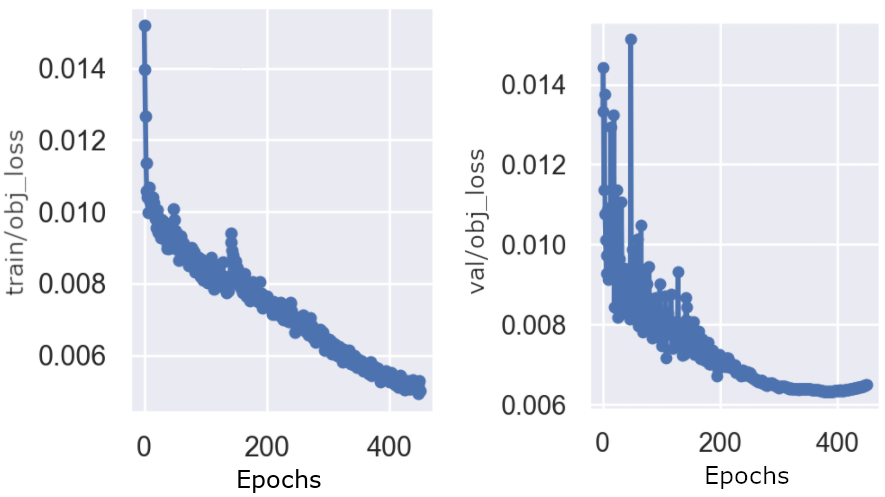
\includegraphics[scale=0.75]{images/train-val-obj-loss.png}
    \caption{The object loss for training and validation data sets over 400 epochs.}
    \label{fig:epochs}
\end{figure}

\subsubsection{Early Stopping}

Performance was monitored on the held-out validation set during training to conditionally terminate the process if over-fitting was detected. This regularisation in time stopped the training after 100 epochs without improvement in validation loss.

\subsubsection{Iterations} 

With a batch size of 32 and 2,559 training images, it would take $\ceil{2,559 / 32} = 80$ iterations for a single epoch.

\subsubsection{Hyperparameter Tuning}

Hyperparameter tuning was performed in an attempt to choose the optimal set of parameters for the model. The YOLOv5 project offers a method of hyperparameter evolution that uses a genetic algorithm for optimisation. This algorithm performs hyperparameter mutation for a set number of evolutions with a 90\% probability and a 0.04 variance to create new offspring based on a combination of the best parents from all previous generations. 

This process was run using the best performing model as a base scenario from which to evolve. The value to maximise, \textit{fitness}, was defined as a weighted combination of metrics: mAP@0.5 contributes 10\% of the weight and mAP@0.5:0.95 contributes the remaining 90\%. A total of 29 hyperparameters are optimised by maximising the fitness. If the metric is greater than the previous evolution, the new offspring is used and the hyperparameter has evolved. 

Due to how expensive this evolution process is only 10 generations were completed. This likely limited its effectiveness as it did not fulfil the recommended minimum of 300 evolutions for best results\cite{yolov5-hyperparam}.

\subsection{Faster R-CNN}

In addition to YOLO-based models, Faster R-CNN models were trained and evaluated for comparison using detectron2\footnote{https://github.com/facebookresearch/detectron2}. These models were created using the same augmented data, batch size and epochs described in previous sections. However, there was no built-in method for automated hyperparameter tuning. Fortunately, as described in chapter \ref{chapter:results}, this would not be necessary as the YOLO-based models were the better performers. After it was discovered that the YOLO models were producing better results, they became the focus of the study to save training time.

\section{Regression}

Count data regression was performed on the modified SIMD data set using generalised linear models to answer the question of interest: Is there a relationship between any of Glasgow City's deprivation indicators, and the amount of litter on its streets?

This data analysis began after a final object detection model had been chosen and applied to quantify the amount of litter within each data zone. The litter count data was added to the SIMD data set as a response variable. An explanation of the object detection results can be found in chapter \ref{chapter:results}. 

\subsection{Data Preparation}

\subsubsection{Data Split}

As we are interested in relationships rather than making predictions we can use the entire data set of 746 observations to obtain more precise estimates than a split would allow. However, as we will be using forward stepwise variable selection to hypothesise the significant explanatory variables, we should set aside a test data set to perform inference. If we do not do this, a train-test leakage will occur as the data will have already been seen by the model building process during feature selection.

The data were split into training and test data sets uniformly at random using an allocation of 80\% and 20\%. The model was trained on the 596 training data observations and the 150 test data observations were used for inference.

\subsubsection{Standardisation} 

Standardisation was performed as many of the features were not recorded on the same scale. For example, the \textit{crime\_rate} was measured in units of per 10,000 people, whereas the \textit{employment\_rate} is the percentage of people who are income deprived. It is important to re-scale the features to be comparable as the interpretation of regression coefficients is sensitive to the scale of the inputs. The Z score standardisation method was applied which produces a mean of zero and a standard deviation of one.

\begin{equation}
    Z = \frac{x - \mu}{\sigma}
\end{equation}

\subsubsection{Missing Data} 

As described in chapter \ref{chapter:data}, 137 missing values were imputed using the mean of the observed values from the other observations. It is important to retain as much information as possible to train with as the data set is small.

\subsection{Exploratory Analysis}

\subsubsection{Correlations}

Figure \ref{fig:correlation-matrix} shows the features of the data that are most positively and most negatively correlated with the response variable. Pearson's correlation coefficient tells us that as \textit{no\_qualifications}, \textit{income\_rate}, \textit{CIF}, \textit{employment\_rate}, \textit{EMERG} and \textit{DEPRESS} increase, so does the amount of the litter. Some of these results may appear counterintuitive, but it is important to remember that these are measures of deprivation i.e., \textit{employment\_rate} is the percentage of employment deprived individuals and not the percentage of employed individuals. Conversely, as \textit{Attainment} and \textit{Attendance} increase, the amount of litter decreases. The strength of these correlations is moderate, suggesting that there may be an association and a relationship with litter. For this reason, these features were used as the explanatory variables from which to construct regression models.

\begin{figure}[h!]
    \centering
    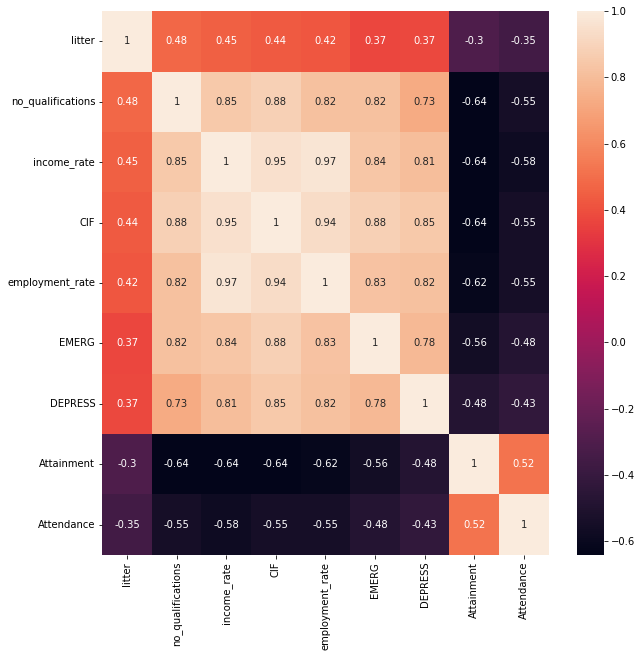
\includegraphics[scale=0.45]{images/corr-matrix.png}
    \caption{The features that were most positively and negatively correlated with litter using Pearson's correlation.}
    \label{fig:correlation-matrix}
\end{figure}

The positively correlated features are deprivation indicators that we would strive to keep low. For example, we would like to minimise \textit{no\_qualifications} as it is the ratio of working-age people with no qualifications. This tells us that we may see litter increase in areas where qualifications are rarer. The same can be said for the other positively correlated features.

On the other hand, the negatively correlated features are related to deprivation indicators that we would like to see maximised. Namely, the percentage of pupils attending school and the attainment score of those leaving school. This tells us that as these decrease, or in other words get worse, the number of litter increases.

It should be noted that a change in one of these explanatory variables is not necessarily an explanation for a change in the amount of litter. Correlation is not causation, and there may be a third yet unidentified causal explanatory variable that both are related to.

\subsubsection{Multicollinearity}

Both \textit{income\_count} and \textit{employment\_count} were also identified as some of the most correlated explanatory variables. However, as they are highly correlated with \textit{income\_rate} and \textit{employment\_rate}, they were omitted from further analysis to avoid issues with multicollinearity. This occurs when the independent variables in the regression model are related. By definition, to be independent variables they should be independent in nature. If not addressed, the resulting regression coefficients may be unstable.

\subsection{Poisson Regression}

The first model $Y \sim Poi(\mu)$ assumes a Poisson distribution where $\mu$ is defined as the number of littered objects detected in fifty street view images. These are the images that were uniformly randomly sampled from a data zone in Glasgow City.

Using the eight explanatory variables identified and described during exploratory analysis, forward stepwise feature selection was performed to identify the features which produced the best fit using the Akaike Information Criterion (AIC) as the selection criteria. With the aim of producing easily an interpretable model, the resulting coefficients are outlined in figure \ref{fig:pos-coeff}.

\begin{figure}[h!]
    \centering
\footnotesize
\begin{verbatim}
=====================================================================================
                        coef    std err          z      P>|z|      [0.025      0.975]
-------------------------------------------------------------------------------------
Intercept             2.2546      0.014    164.731      0.000       2.228       2.281
Attainment            0.0277      0.018      1.534      0.125      -0.008       0.063
Attendance           -0.0764      0.017     -4.606      0.000      -0.109      -0.044
EMERG                -0.0984      0.026     -3.845      0.000      -0.149      -0.048
DEPRESS               0.0775      0.025      3.140      0.002       0.029       0.126
employment_rate      -0.1621      0.051     -3.180      0.001      -0.262      -0.062
CIF                  -0.0601      0.051     -1.183      0.237      -0.160       0.039
income_rate           0.2930      0.059      5.003      0.000       0.178       0.408
no_qualifications     0.2869      0.027     10.530      0.000       0.233       0.340
=====================================================================================
\end{verbatim}
\normalsize
    \caption{The coefficients of the Poisson regression model using the training data.}
    \label{fig:pos-coeff}
\end{figure}

Only the \textit{Attainment} and \textit{CIF} features failed to produce a p-value less than significance threshold $\alpha = 0.05$. However as the model fit is poor, we cannot conclude that there are any significant relationships.

As the variance in GLMs are not constant but vary with the mean, we cannot rely on the raw response residuals to assess model fit. The variance is equal to the mean for the Poisson model therefore we use the Pearson chi-squared statistic instead. The Pearson statistic is $\chi^2 = 2158$ which is very large when compared to the $\chi^2(587)$ distribution, indicating a poor fit if the Poisson is the correct model for the response.

\subsubsection{Overdispersion}

If the assumption that the variance is equal to the mean does not hold then overdispersion may occur. This is a potential explanation for the poor model fit as while the regression parameter estimates are consistent, their standard errors will be incorrect. For this reason, models which do not make this assumption were developed.

\subsection{Negative Binomial Regression}

The next model $Y \sim NegBin(\mu, \alpha)$ introduces a dispersion parameter $\alpha$ and assumes a Negative Binomial distribution for the response which allows for a variance larger than the mean.

Once again, using the eight explanatory variables identified during exploratory analysis, forward stepwise feature selection was performed using AIC. The resulting coefficients are outlined in figure \ref{fig:nb-coeff}.

The only coefficients that may be statistically significant, where $p < 0.05$, are \textit{Attendance}, \textit{income\_rate} and \textit{no\_qualifications}.

The Pearson statistic is $\chi^2 = 432$ which is smaller than the $\chi^2(587)$ distribution, indicating that the model fits if the Negative Binomial is the correct model for the response.

\begin{figure}[h]
    \centering
\footnotesize
\begin{verbatim}
=====================================================================================
                        coef    std err          z      P>|z|      [0.025      0.975]
-------------------------------------------------------------------------------------
Intercept             2.2536      0.029     76.866      0.000       2.196       2.311
Attainment            0.0159      0.040      0.392      0.695      -0.063       0.095
Attendance           -0.0784      0.037     -2.100      0.036      -0.152      -0.005
EMERG                -0.0994      0.063     -1.589      0.112      -0.222       0.023
DEPRESS               0.0427      0.057      0.745      0.457      -0.070       0.155
employment_rate      -0.1950      0.122     -1.602      0.109      -0.434       0.044
CIF                  -0.0606      0.123     -0.494      0.622      -0.301       0.180
income_rate           0.3407      0.140      2.437      0.015       0.067       0.615
no_qualifications     0.2962      0.065      4.588      0.000       0.170       0.423
=====================================================================================
\end{verbatim}
\normalsize
    \caption{The coefficients of the Negative Binomial regression model using the training data.}
    \label{fig:nb-coeff}
\end{figure}

\subsubsection{The Reproducibility Crisis}

More than 70\% of researchers have tried and failed to reproduce another scientist's experiments, and more than half have failed to reproduce their own experiments\cite{Baker2016}. One of the leading factors that contribute to such outcomes is \textit{p-hacking}: the process of re-examining the data until a statistically significant effect is observed. It is important to mitigate against this multiple testing to avoid concluding that a result is significant through random chance.

\subsubsection{Bonferroni Correction}

The multiple testing problem describes the fact that as our number of tests for significant effects increases, so does the likelihood of a false positive arising. To mitigate against this, Bonferroni Correction was applied to guard against the bias of repeated testing effects. The coefficient p-values were adjusted such that they are unlikely to be significant through random chance. This divides the significance level $\alpha = 0.05$ by the number of tests, which has the unfortunate side effect of decreasing the likelihood that a true effect is detected when true.

After applying Bonferroni Correction \textit{no\_qualifications} was the only remaining significant explanatory variable. However, we cannot conclude from this as we must further test our variable selection hypothesis using the test data set.

% Results =====================================================================

\chapter{Results} \label{chapter:results}

\section{Litter Detection}

A comparison was performed between the results of each trained object detection model to choose a final model that would be used to infer the litter counts in each data zone.

\subsection{Model Selection}

The standard evaluation metric to use for model selection is the mean average precision (mAP), which quantifies the performance of an object detector across all validation images and at different confidence thresholds.

\begin{table}[ht!]
    \centering
    \begin{tabular}{|l| |l|} 
     \hline
     \textbf{Model} & \textbf{mAP} \\
     \hline\hline
     YOLOv5s with Mosaic x3, 5\% Noise and Tuned & 58.2 \\
     YOLOv5s with Mosaic x3 & 53.0 \\
     YOLOv5s with Mosaic x3, 5\% Noise & 43.6 \\
     YOLOv5s with Mosaic x3, Auto-adjust Contrast, 5\% Noise & 42.1 \\
     YOLOv5s with Mosaic x2 & 40.9  \\
     YOLOv5s with Mosaic x2, Auto-adjust Contrast & 40.1  \\
     YOLOv5s with No Augmentations & 38.6 \\
     Faster R-CNN with Mosaic x3 & 39.5 \\
     Faster R-CNN with No Augmentations & 26.5 \\
     \hline
    \end{tabular}
    \vspace{2mm}
    \caption{The mean average precision (mAP 0.5-0.95) results for the trained object detection models on the validation data.}
    \label{table:model-mAP}
\end{table}

The hyperparameter tuned YOLOv5s model trained on mosaic and noise augmented data produced the best result with an mAP of 58.2. The precision-recall curve in figure \ref{fig:pr-curve} does a good job at staying close to the upper right corner, maintaining both high precision and high recall values. The high precision means that the model can be trusted when it identifies an object as litter. Similarly, high recall means it also classifies the majority of litter correctly.

\begin{figure}[h!]
    \centering
    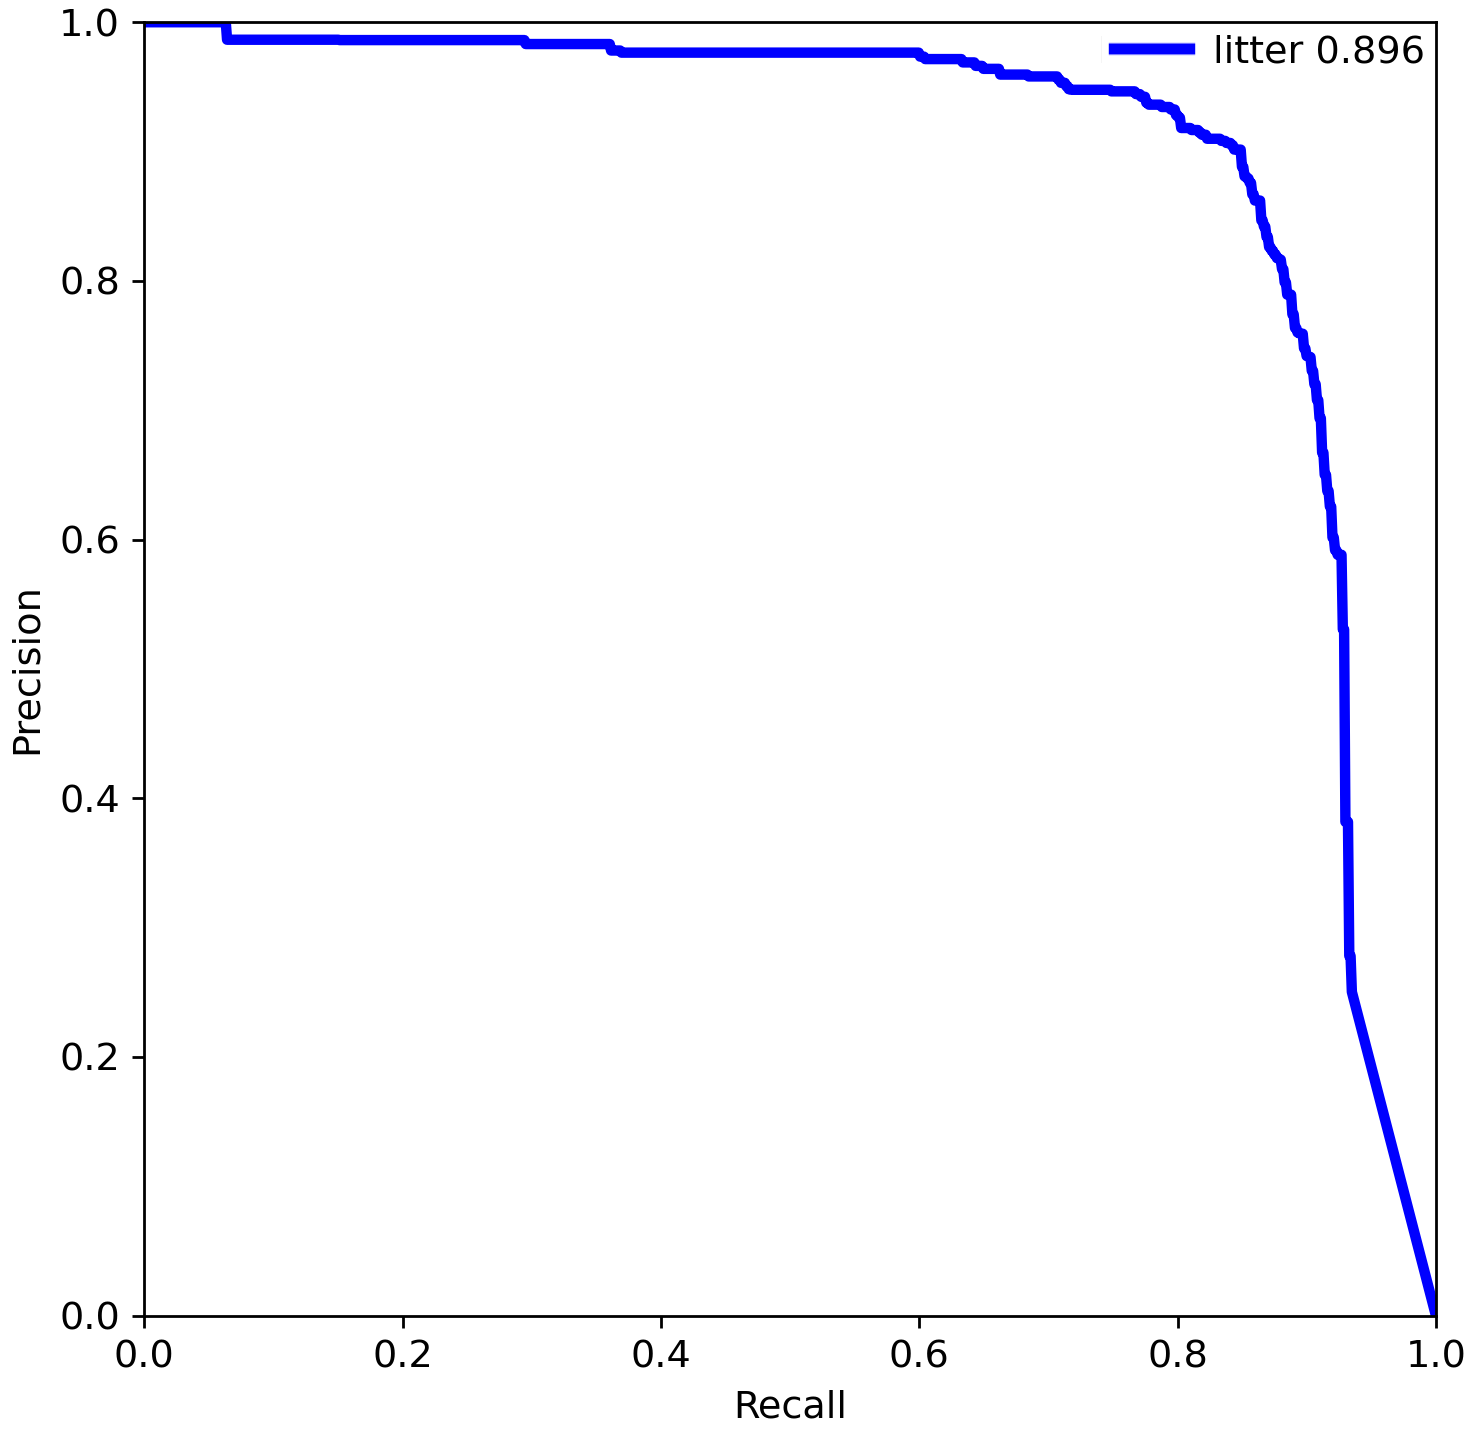
\includegraphics[scale=0.5]{images/pr-curve.png}
    \caption{The precision-recall curve of the chosen model applied to the validation data.}
    \label{fig:pr-curve}
\end{figure}

\begin{figure}[h!]
    \centering
    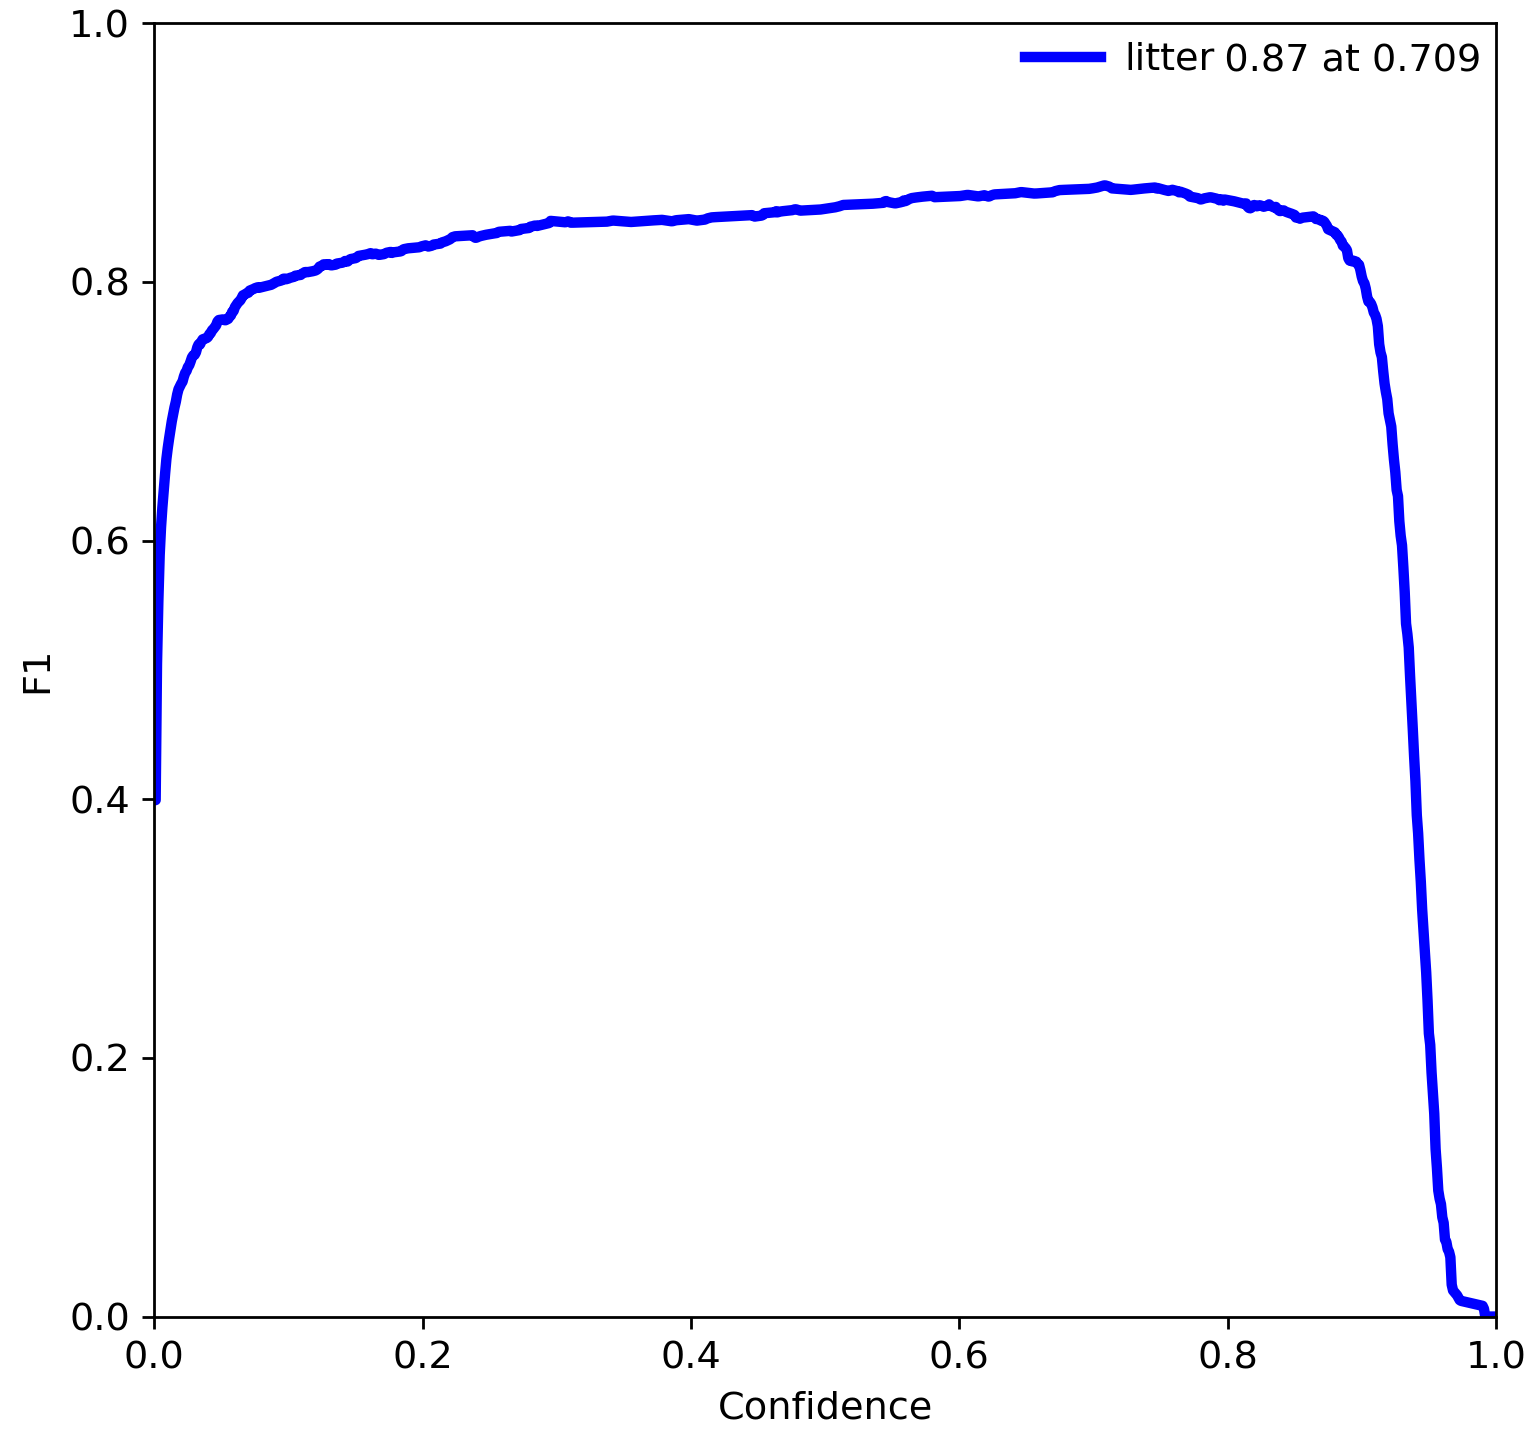
\includegraphics[scale=0.5]{images/f1-curve.png}
    \caption{The F1 curve of the chosen model applied to the validation data.}
    \label{fig:f1-curve}
\end{figure}

The F1 curve shows that the ideal confidence threshold that maximises the F1 metric to 0.87 is 0.709. This is the threshold at which both precision and recall are maximised.

Using a confidence threshold of 80\%, the model performed with a 78\% true positive rate. This means that just under 8 of every 10 occurrences of litter were correctly identified as litter. With a 22\% false negative rate, just over 1 in 5 objects were incorrectly classified as not litter when they should have been. Out of 485 labels, 380 were true positives and 105 were false negatives. A further 36 objects were detected as false positives.

As it produced the best mAP and detected a majority of true positives with few false positives, it was the model chosen to perform the litter quantification of each data zone of Glasgow City.

\subsection{Model Inference}

The chosen YOLO model was used to detect litter using a confidence threshold of 80\%. This threshold was chosen as it was high enough to prevent a lot of false positives while the validation data suggested it would provide an F1 score close to the maximum.

\subsubsection{Application To Glasgow City}

When applied to the 37,300 images collected within Glasgow City's data zones, 7,732 littered objects were detected. Figure \ref{fig:litter-histogram} shows the number of littered objects detected within fifty uniformly randomly sampled images for each data zone. The count ranges from 0 -- 58 littered objects and the average number per data zone was 10. As these counts are an aggregation over fifty images, less than 40 data zones recorded no litter. Software was developed to add these counts to the SIMD data set as a response variable in preparation for regression.

Figure \ref{fig:4-in-bush} is an example of the model performing well. It has successfully detected every piece of litter in the image with good accuracy. 

On the other hand, the model is certainly not perfect. Figure \ref{fig:sandbag} shows that it struggles to differentiate between what looks like litter and what truly is. The sandbags holding up this road sign may look like a plastic bag on the pavement, but the model is unable to use the surrounding context to know the difference.

\newpage
\newgeometry{top=3cm, bottom=1cm}
\begin{figure}[h!]
    \centering
    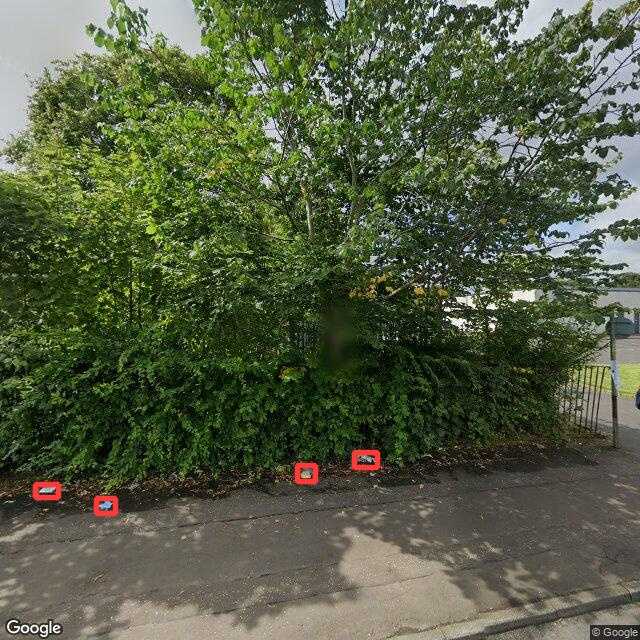
\includegraphics[scale=0.45]{images/good-4-in-bush.jpg}
    \caption{Litter detection example: Four littered objects in a bush.}
    \label{fig:4-in-bush}
\end{figure}

\begin{figure}[h!]
    \centering
    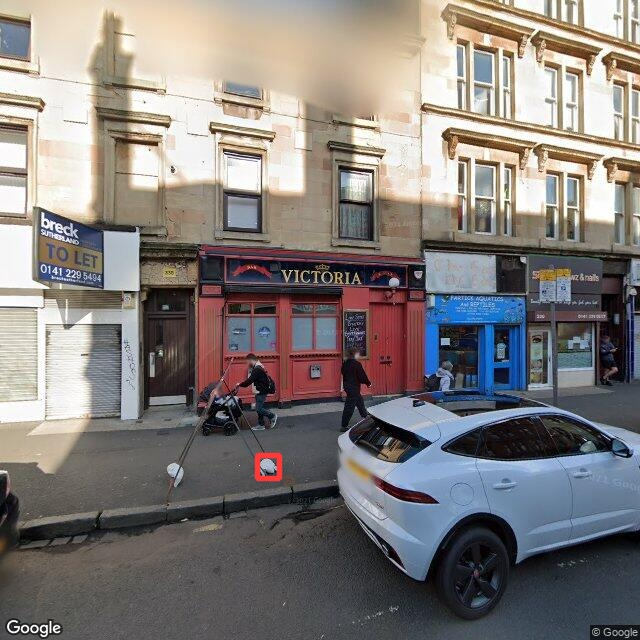
\includegraphics[scale=0.45]{images/flaw-sandbag.jpg}
    \caption{Litter detection example: A white sandbag next to the kerb.}
    \label{fig:sandbag}
\end{figure}
\newgeometry{top=3cm, bottom=3cm}
\newpage

\begin{figure}[h!]
    \centering
    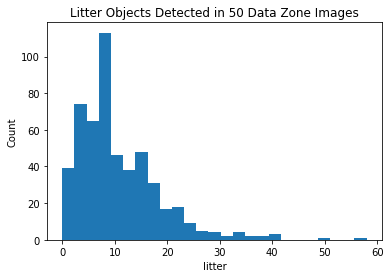
\includegraphics[scale=0.6]{images/litter-hist.png}
    \caption{The number of detected littered objects in each data zone.}
    \label{fig:litter-histogram}
\end{figure}

\subsubsection{Location Generalisation}

The chosen model had a 77\% true positive rate and a 23\% false-negative rate when applied to the test data. Out of 254 labels, 196 were true positives and 58 were false negatives. A further 28 objects were detected as false positives. We should expect one out of every four littered objects to be overlooked by the model. This rate is slightly worse than the result produced using the validation data, but not by much, suggesting that the model may generalise well to unseen data. However, this assumption only holds if the unseen data comes from a location with a similar appearance to Glasgow City. A city's climate and culture will determine its appearance on a street view image. San Francisco does not look the same as Glasgow, and it may not have the same litter.

\begin{figure}[h!]
    \centering
    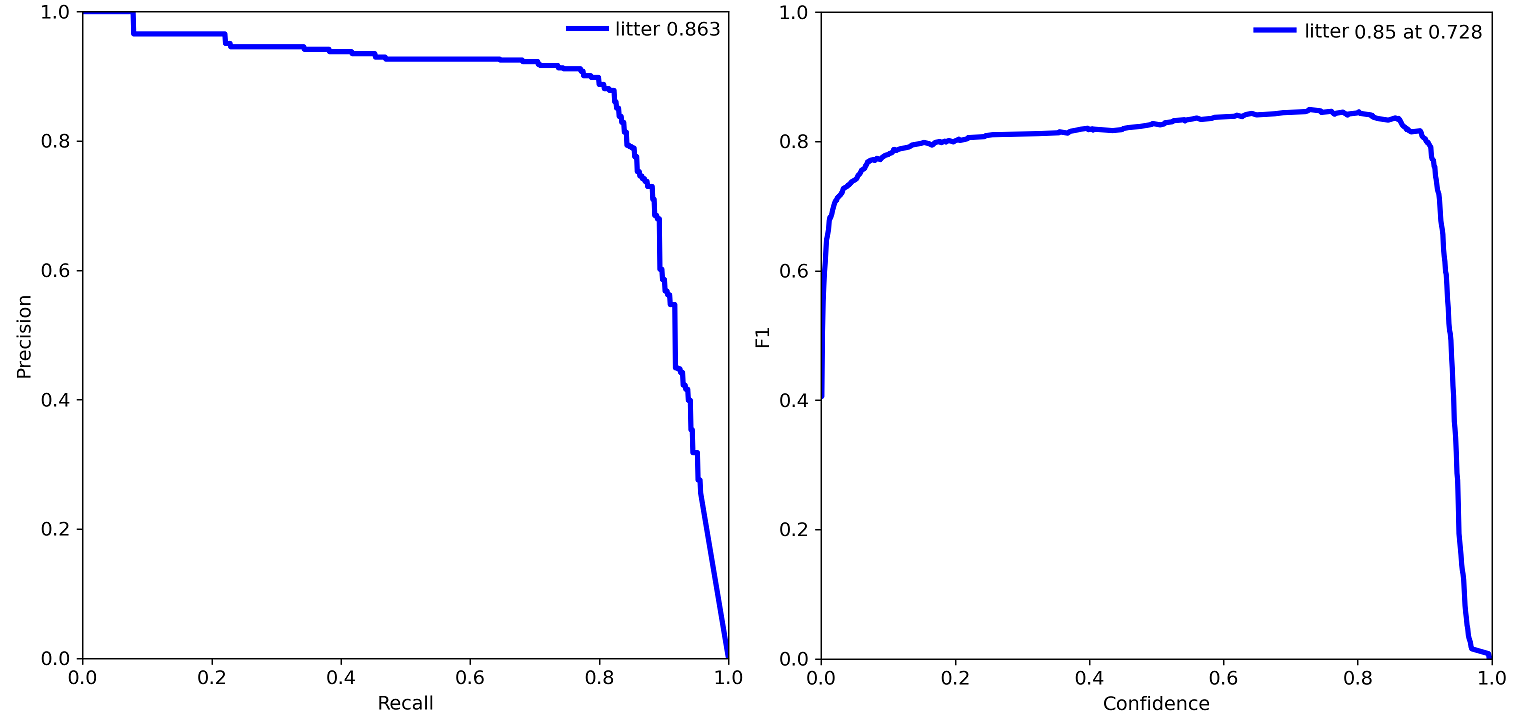
\includegraphics[scale=0.3]{images/fm-prf1-curves.png}
    \caption{The precision-recall and F1 curves of the chosen model applied to the test data.}
    \label{fig:fm-prf1-curve}
\end{figure}

Figure \ref{fig:fm-prf1-curve} shows that the model can maintain high precision and recall in which it both accurately detects only litter, while also detecting the majority of it. The maximum F1 metric of 0.85 reinforces this result and it is achieved when the confidence threshold is set to 0.728.

Figure \ref{fig:4-in-bush} is also a good example of the litter detection model working well. It has successfully identified four small littered objects in the scene, without false positives or false negatives. However, it is certainly not perfect and may detect unexpected objects as litter if they appear similar enough. Figure \ref{fig:sandbag} shows the failings of the model as it detects a white roadside sandbag as litter.


\newpage
\section{Regression}

\subsection{Model Selection}

The Poisson model did not produce an adequate goodness-of-fit statistic on the training data. However, the Negative Binomial model did. For this reason, it was selected as the final model. Figure \ref{fig:predicted-vs-actual-test} shows that although our Pearson chi-squared statistic suggests a good fit when applied to the test data the model does not produce very accurate results. We would expect to see a linear straight line where $X = Y$ if the fit was perfect.

\begin{figure}[h!]
    \centering
    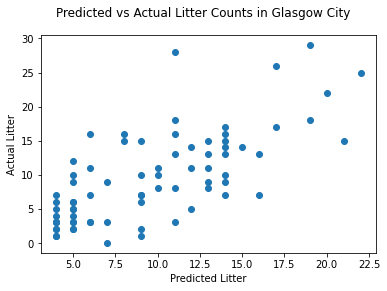
\includegraphics[scale=0.6]{images/predicted-vs-actual-test.png}
    \caption{The predicted litter counts vs the actual counts for the test data.}
    \label{fig:predicted-vs-actual-test}
\end{figure}

\subsection{Relationships}

The chosen model was applied to an unseen data set to test the variable selection hypothesis that the forward stepwise process produced. We cannot use the entire data set, as a hypothesis suggested by a given data set, when tested with the same data set that suggested it, is likely to be accepted even when is untrue\cite{testing-hyp-wikipedia}.

Applying the chosen model to the test data produces the coefficients shown in Figure \ref{fig:nb-coeff-test}. None of the explanatory variables are statistically significant with a p-value less than $\alpha = 0.05$. This suggests there are no relationships between these indicators of deprivation and the amount of litter.

\begin{figure}[h!]
    \centering
\footnotesize
\begin{verbatim}
=====================================================================================
                        coef    std err          z      P>|z|      [0.025      0.975]
-------------------------------------------------------------------------------------
Intercept             2.3226      0.058     39.977      0.000       2.209       2.436
Attainment           -0.1023      0.080     -1.280      0.201      -0.259       0.054
Attendance            0.0513      0.087      0.592      0.554      -0.118       0.221
DEPRESS              -0.0392      0.109     -0.358      0.720      -0.254       0.175
EMERG                 0.0680      0.146      0.464      0.642      -0.219       0.355
employment_rate      -0.0432      0.221     -0.195      0.845      -0.476       0.390
CIF                   0.0485      0.219      0.222      0.824      -0.380       0.477
income_rate           0.2212      0.254      0.871      0.384      -0.277       0.719
no_qualifications     0.1235      0.168      0.737      0.461      -0.205       0.452
=====================================================================================
\end{verbatim}
\normalsize
    \caption{The coefficients of the Negative Binomial regression model using the test data.}
    \label{fig:nb-coeff-test}
\end{figure}

The Pearson statistic is $\chi^2 = 107$ which is smaller than the $\chi^2(141)$ distribution, indicating that the model fits if the Negative Binomial is the correct model for the response. However, figure \ref{fig:predicted-vs-actual-test} shows some wide residuals between the predicted and actual litter counts that indicate that it does not perform very well.

\chapter{Software}

In addition to data analysis, this study includes an extensive software component. A companion web application was developed to provide a user-friendly way of exploring the litter detection results.

\begin{figure}[h]
    \centering
    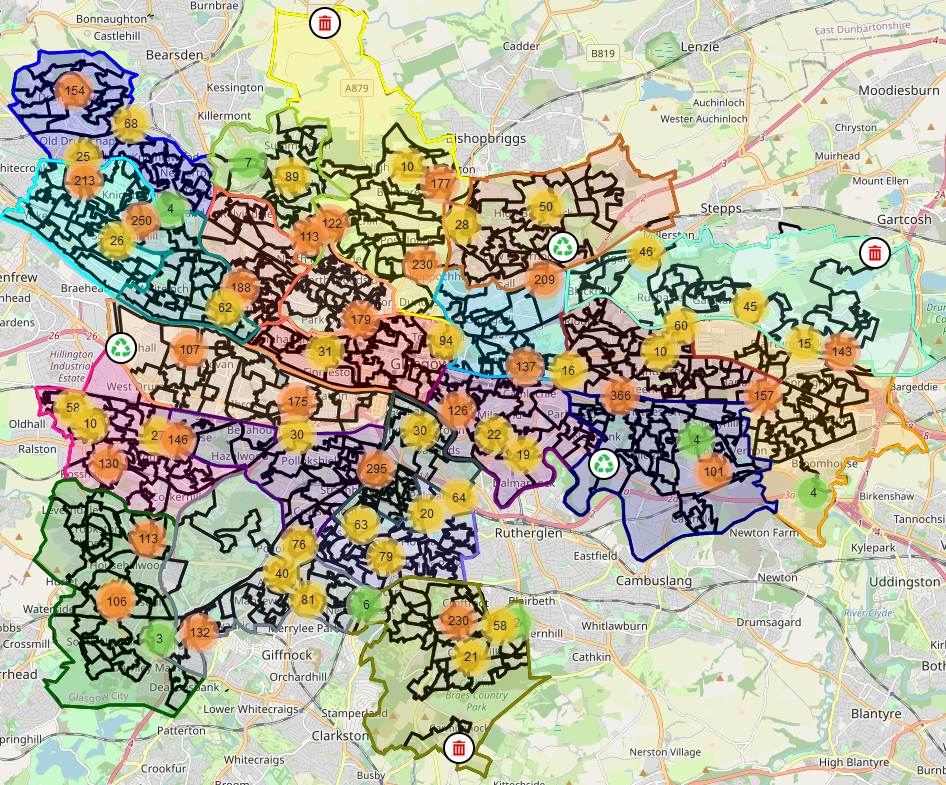
\includegraphics[scale=0.40]{images/glasgow-city.PNG}
    \caption{The interactive litter cluster data visualisation of Glasgow City.}
\end{figure}

It includes an interactive map visualisation of Glasgow City with the detected litter marked within well-defined city ward and data zone boundaries. Users can click on a marker to view the image with the bounding boxes that have been produced by the detector. Marker clusters are split and combined as the user zooms in and out of the visualisation. Markers for the public recycling facilities are also available and the visibility of all elements is toggle-able. By displaying only the litter marker clusters, users can see at a glance which areas of the city have the highest concentration of litter. The resulting visualisation shows that the central areas of the city have many more instances of detected litter than those in the south.

The application also allows users to upload their own street view images to run against the final litter detection model. A confidence threshold slider is included to easily test how different the results are at different levels. Options to set the visibility of bounding boxes and confidence values are also available. This feature allows users to test the usefulness of the model by providing their own unseen data.

Individuals from local groups who are interested in tracking the cleanliness of Glasgow City may find this useful. Members of organisations such as Keep Scotland Beautiful and Glasgow City Council would be able to assess the prevalence of litter in different areas. With further improvements, such as periodically updating the data displayed, there is potential for it to aid policy-making decisions.

The software was developed using the React JavaScript framework, HTML, and CSS. This is backed by a Python service that facilities the running of the object detector. The web application is hosted on a virtual private server and is publicly accessible at \url{https://glasgow-litter.garyblackwood.co.uk}. The source code is open source and persists on \url{https://github.com/Garee/glasgow-litter}.


% Discussion ==================================================================

\chapter{Discussion}

\section{Recommendations}

It was of interest to discover relationships between the key indicators of deprivation in Glasgow City and the amount of litter on its streets. Although the regression analysis produced a model that fits the data, the findings were unable to identify any statistically significant explanatory variables. Looking solely at the training data results, it did appear that an increase in the number of working-age individuals without qualifications would also see the amount of litter in that area increase. If true, it would be sensible to recommend that the government focus on helping the citizens attain qualifications if they also wish to tackle litter. However, the test data results were unable to confirm this conclusion, as it was found not to be statistically significant enough to advise.

A manual human audit is currently the primary means of assessing urban cleanliness. Organisations such as Keep Scotland Beautiful carry out annual local environmental quality surveys at a random selection of sites across Scotland every year\cite{leams}. In the 2020/21 audit, the organisation assessed 10,869 individual sites across 71 areas in Scotland. The automated approach taken in this study was able to assess tens of thousands of images in Glasgow City alone. The good performance of the detector on the held-out test data gives confidence to the idea that it can be applied across the country. With substantially more data at their fingertips, organisations would be able to improve their audits and recommendations. There is the potential for cost savings if the capital needed to obtain the images is less than any human resources.

These findings are not conclusive. The challenges of limited scope, data quality, data quantity, time, and hardware resources, could all be overcome to improve the accuracy and reliability of the results.

\section{Limitations and Future Work}

\subsection{Image Resolution}

Detecting small objects is a challenging problem in computer vision. In YOLOv4 for example, the mean average precision on small objects was only 20.4\% in comparison to 56\% for large\cite{yolov4}. This is almost a three-fold difference in performance.

Littered objects are generally very small and only take up a tiny proportion of the overall pixel count of an image. During training, a model does not have much information to work with for this reason. This problem is compounded when the input image resolution size is low.

This study was limited to a maximum image resolution of 640x640 pixels as this was the largest size offered by the Google Street View API. Obtaining larger images could produce better performing models as the increased fidelity provides more data to learn from. Furthermore, it would also allow different types of littered objects to be identified. This study was limited to a single \textit{litter} class, as the objects were too small to accurately classify any further. Policy-making decisions could be improved if we knew what types of litter are most prevalent.

\subsection{Time and Hardware}

An input image that is twice as large requires the CNN to learn from four times as many pixels. The additional time needed to learn adds up quickly unless more hardware resources are made available to compensate. This study used a personal computer with consumer graphics card acceleration and a relatively small number of model parameters to keep the training time reasonable. For example, the YOLOv5x model has 86.7 million parameters in comparison to the YOLOv5s model's 7.2 million. Even with this approach, the development of a single model still took many hours. The time constraint also limited how many generations the hyperparameter tuning genetic algorithm was able to complete. Additional hardware resources would allow larger models to be developed and tuned for better performance. The YOLOv5x model provides better results in nearly all cases\cite{better-training-results}. Applying this model would be a straightforward way to improve the results described. The trade-off would be less time for higher capital costs, as expensive GPUs would need to be purchased or rented.

\subsection{Out of Sight Areas}

Every image used for training and inference was collected from Google street view. These images are obtained by Google using a car with a 360-degree camera on its roof. This means that the models developed in this study were only able to learn and infer from areas visible from the road. Litter in alleyways, back gardens, parks, and any area inaccessible by car would not be taken into account. It is important to consider that there may be a significant amount of litter not visible from the road. Further work could explore applying this approach to these areas.

\subsection{Zero Inflated Models}

As roughly one in twenty data zones had zero littered objects detected within them, a zero-inflated model may produce better regression results. This type of statistical model is based on a distribution that allows for frequent zero-valued observations. It allows for a separate statistical process to determine the zero and non-zero counts. Both Poisson and Negative Binomial models have zero-inflated variants that allow for overdispersion and could be applied and evaluated.

\subsection{Longitudinal Analysis}

By applying these methods over time, it is possible to track whether progress is being made or not in the effort to reduce littering. Local government services could retrofit their bin collection vehicles to collect images regularly for the purpose of quantifying the amount of litter using object detection. Time series analysis methods could be applied to extract trends in the data. The findings could help policy-makers make informed choices.

\subsection{Spacial Analysis}

The first law of geography states that nearer things are more related to each other than distant things\cite{law-geog-wikipedia}. Therefore, it is unlikely that the amount of litter is randomly distributed across the data zones in Glasgow City. In this case, the data is said to be auto-correlated. It, unfortunately, means that the assumption that the data is statistically independent is violated. One data zone in the training set and another data zone in the validation set may be very similar to each other as they are neighbouring, even though they were randomly sampled during the data split. This increases the likelihood of overfitting. To address this problem, a future analysis could group the data by area to prevent the model from looking at data it should not. The results of the Poisson and Negative Binomial models developed may be less reliable due to the presence of spatial effects in the data.

\subsection{Software}

Enhancements to the companion web application could be made to increase the amount of training data available. The quantity of data was limited due to the need to hand annotate the images. The ability to annotate these images could be added to the software such that the task could be crowdsourced. If added, the new problem of annotation reliability would need to be addressed. The Trash Annotations in Context project released a similar feature to its website\footnote{http://tacodataset.org/annotate}.

\section{Conclusion}

This study aimed to identify the relationships between the key indicators of deprivation in areas of Glasgow City and the amount of litter on its streets. Initial exploratory data analysis suggested that these relationships may indeed exist. However, after performing count data regression it was discovered that none of the potential explanatory indicators were statistically significant at $\alpha = 0.05$, even though the goodness-of-fit statistic for the regression model met the required threshold.

It was also of interest to discover if an automated approach to counting litter on a city-scale could be achieved using deep learning object detection methods. A YOLOv5s object detection model was developed to detect litter within Google street view images of Glasgow City. After confirming the feasibility of collecting such images at a large scale, the model was successfully applied to 37,300 images. The results establish that there is good potential for this approach to be scaled up. Scaling may include increasing the number of images the model is applied to, the number of locations it is used for, and the frequency of application. Furthermore, by holding out a test data set that produced a 77\% true positive rate over 254 littered objects, it was discovered that the detection model generalises reasonably well to new data.

Litter is undoubtedly an important indicator of environmental quality\cite{household-survey-2019}. Even though no link with deprivation could be established presently, if local organisations were able to apply these methods throughout the country, perhaps progress could be made in reducing litter and discovering its causes. This would be a welcome step towards a cleaner world.

% Appendices ==================================================================

\begin{appendices}

\chapter{Litter Detection Examples}

\begin{figure}[h!]
    \centering
    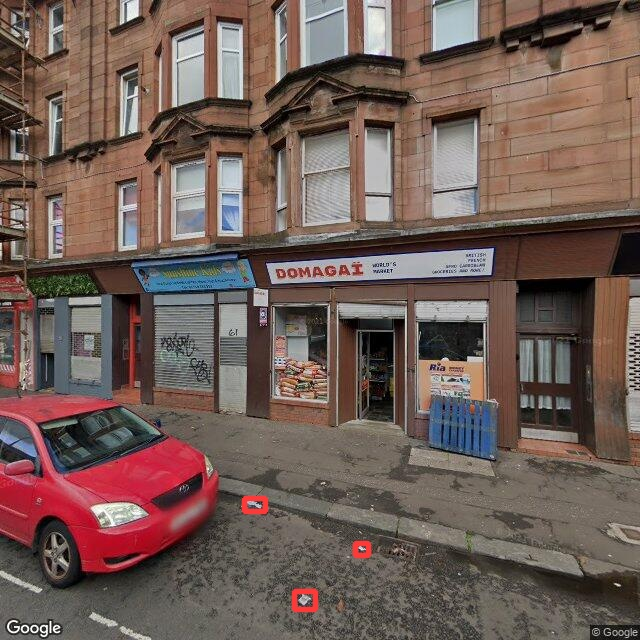
\includegraphics[scale=0.5]{images/good-three.jpg}
    \caption{Litter detection example: A few littered objects next to the pavement.}
\end{figure}

\begin{figure}[h!]
    \centering
    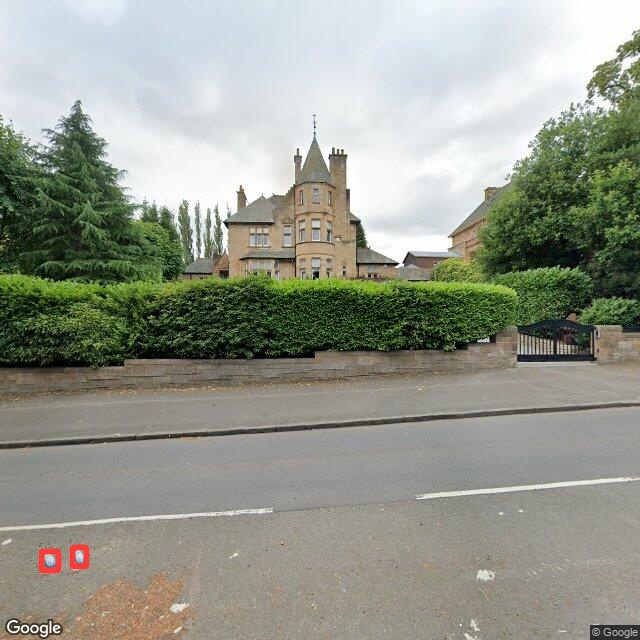
\includegraphics[scale=0.5]{images/good-two-bottles.jpg}
    \caption{Litter detection example: Two plastic bottles on the road.}
\end{figure}

\begin{figure}[h]
    \centering
    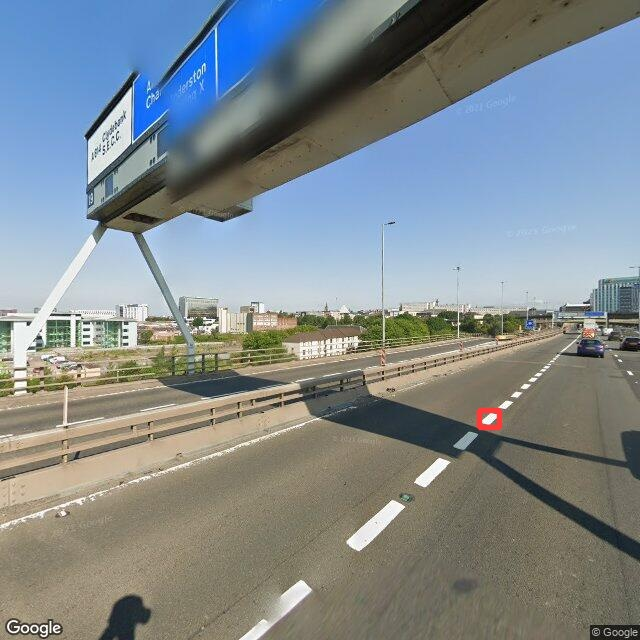
\includegraphics[scale=0.5]{images/flaw-road-marking.jpg}
    \caption{Litter detection example: A white lane separator road marking.}
\end{figure}

\begin{figure}[h]
    \centering
    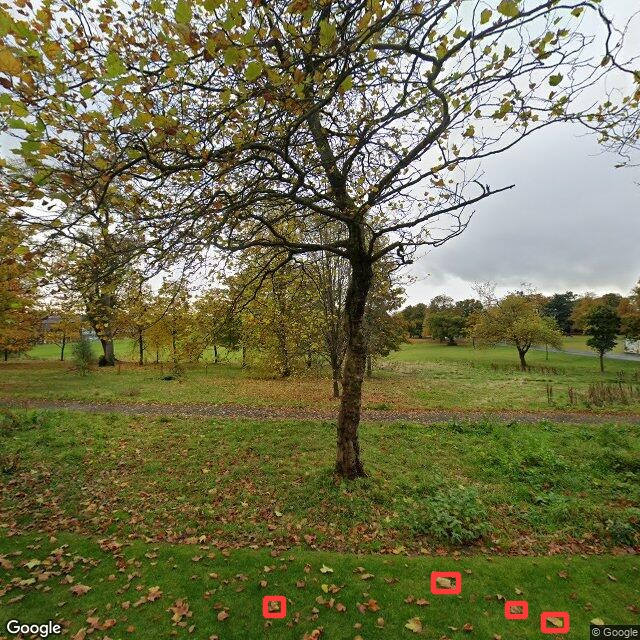
\includegraphics[scale=0.5]{images/flaw-tree-leaves.jpg}
    \caption{Litter detection example: Leaves that have fallen from a nearby tree.}
\end{figure}

\chapter{Litter Detection Confusion Matrices}

\begin{figure}[h!]
    \centering
    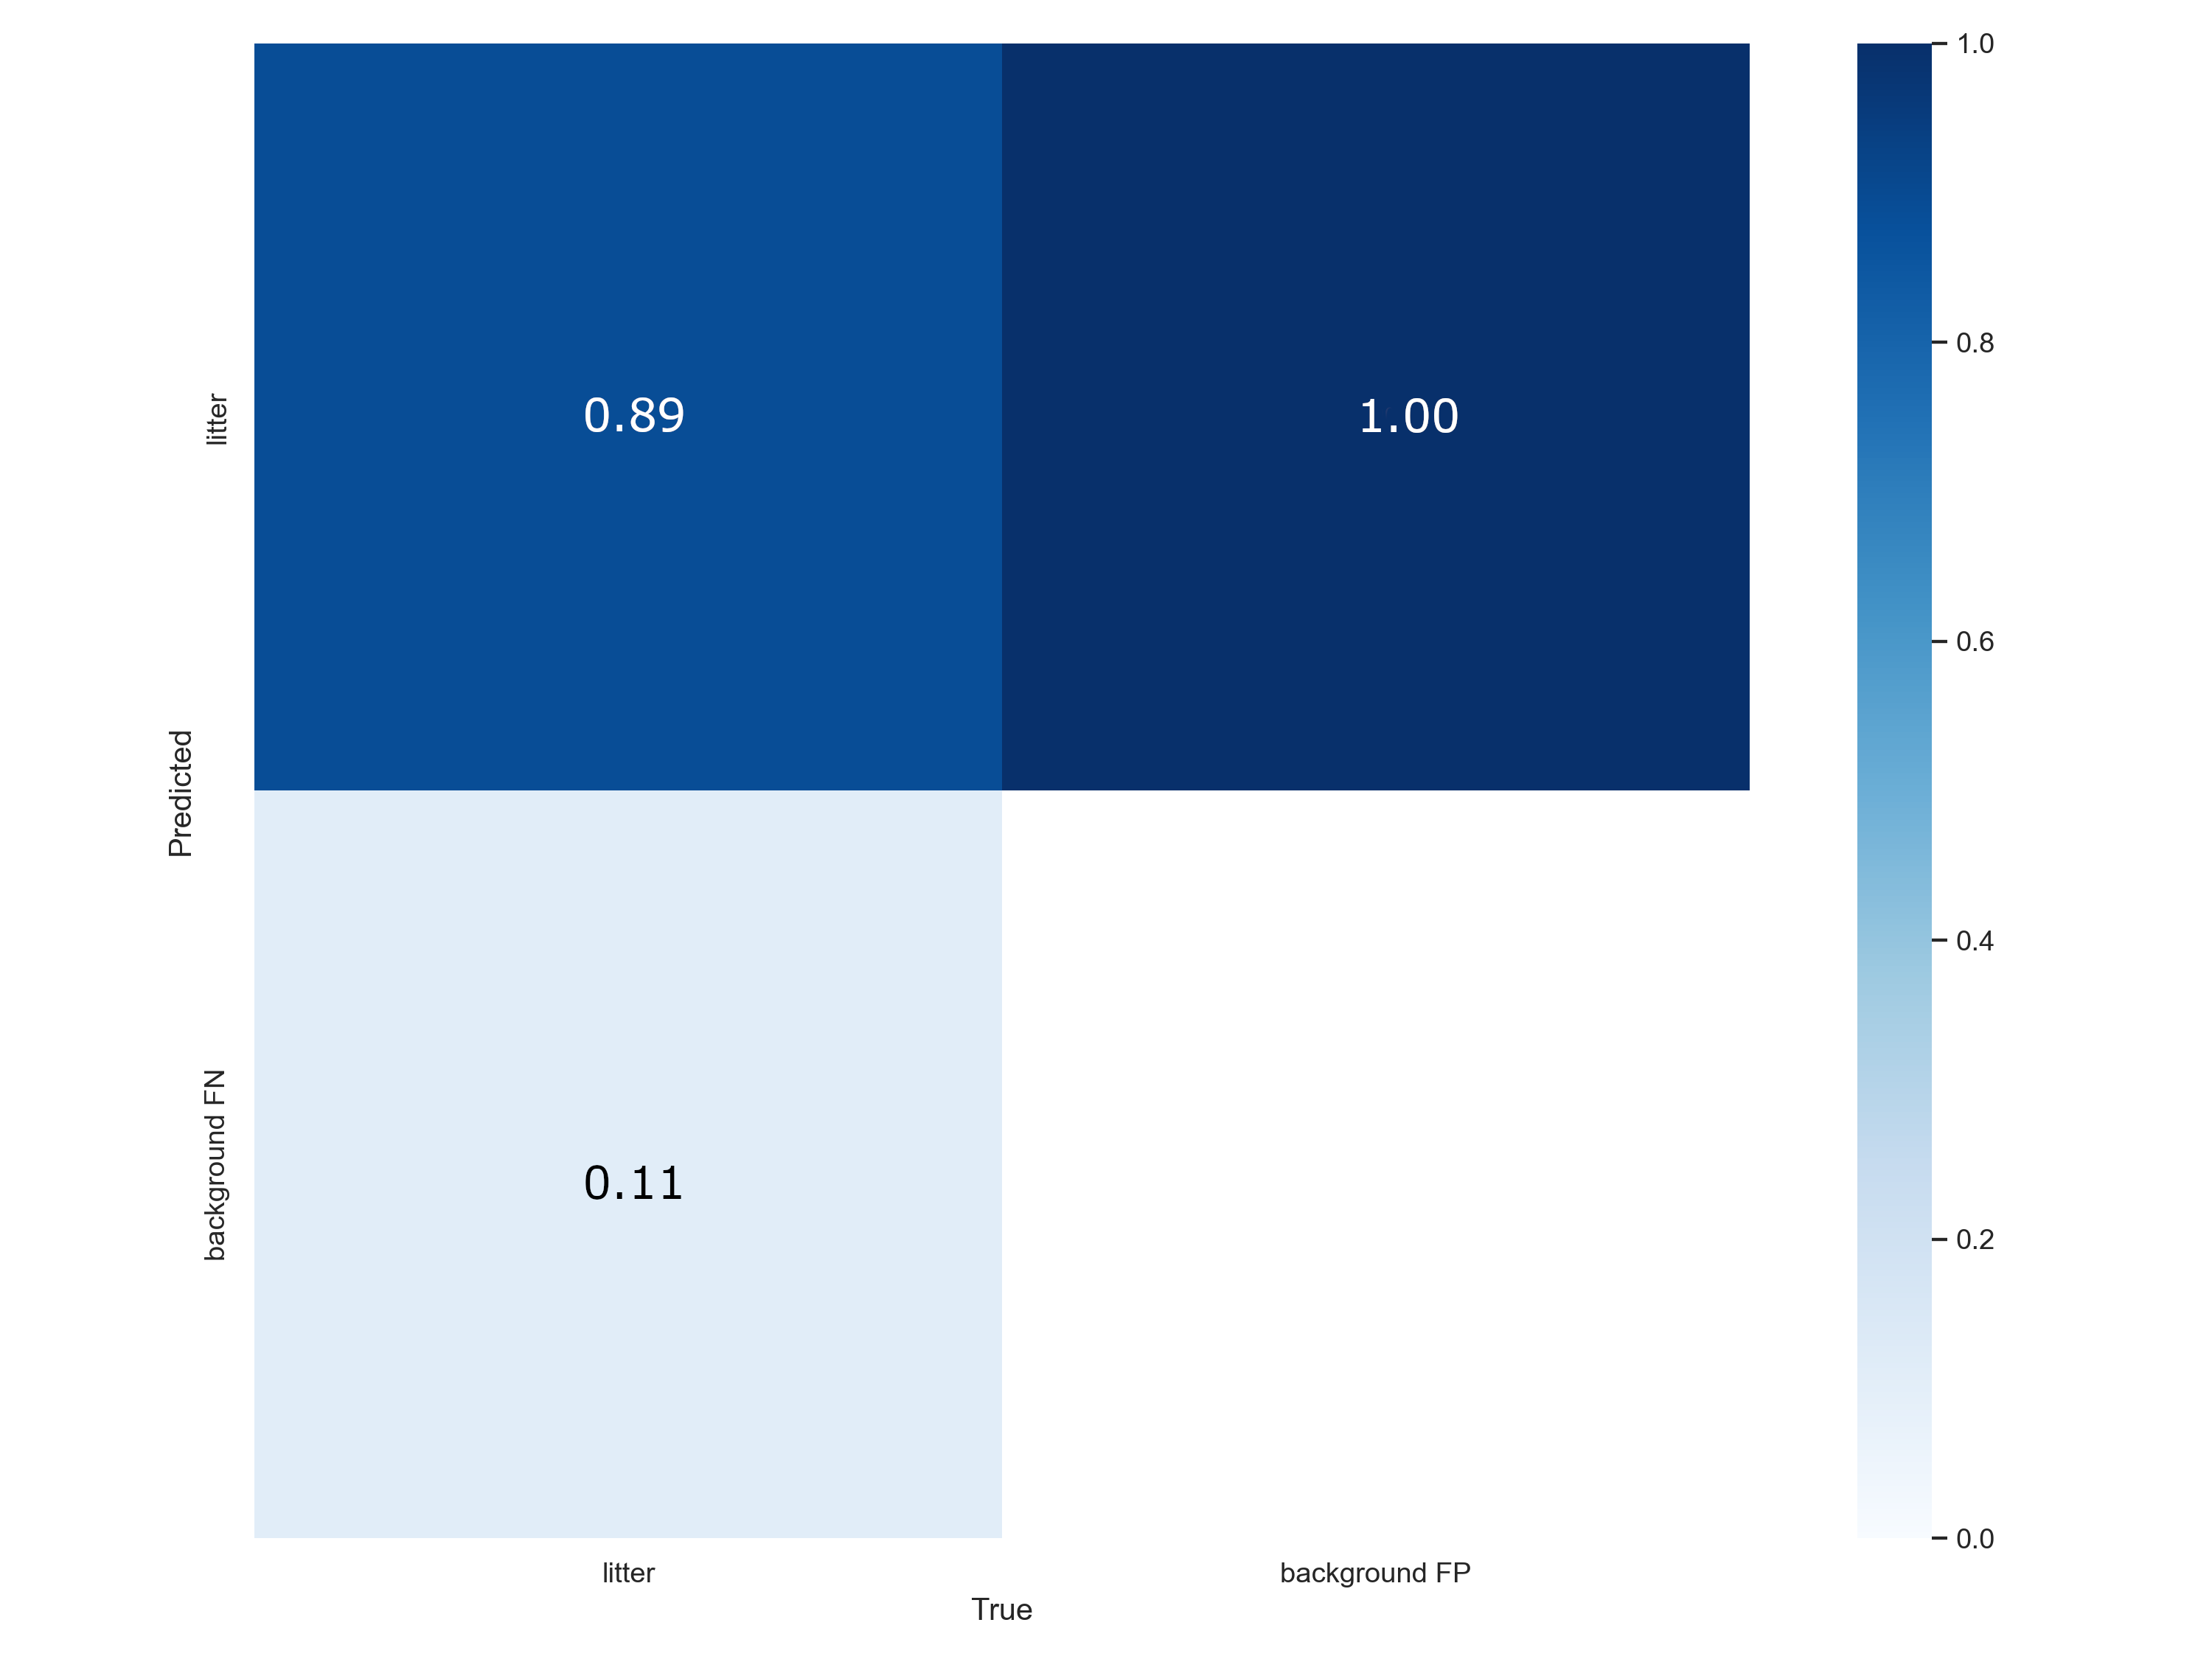
\includegraphics[scale=0.5]{images/final-model-confusion-matrix-val.png}
    \caption{The confusion matrix of the litter detection model when applied to the validation data. This shows a 78\% TPR, 22\% FNR, and tells us that every false positive was a member of the litter class.}
    \label{fig:confusion-matrix-validation}
\end{figure}

\begin{figure}[h!]
    \centering
    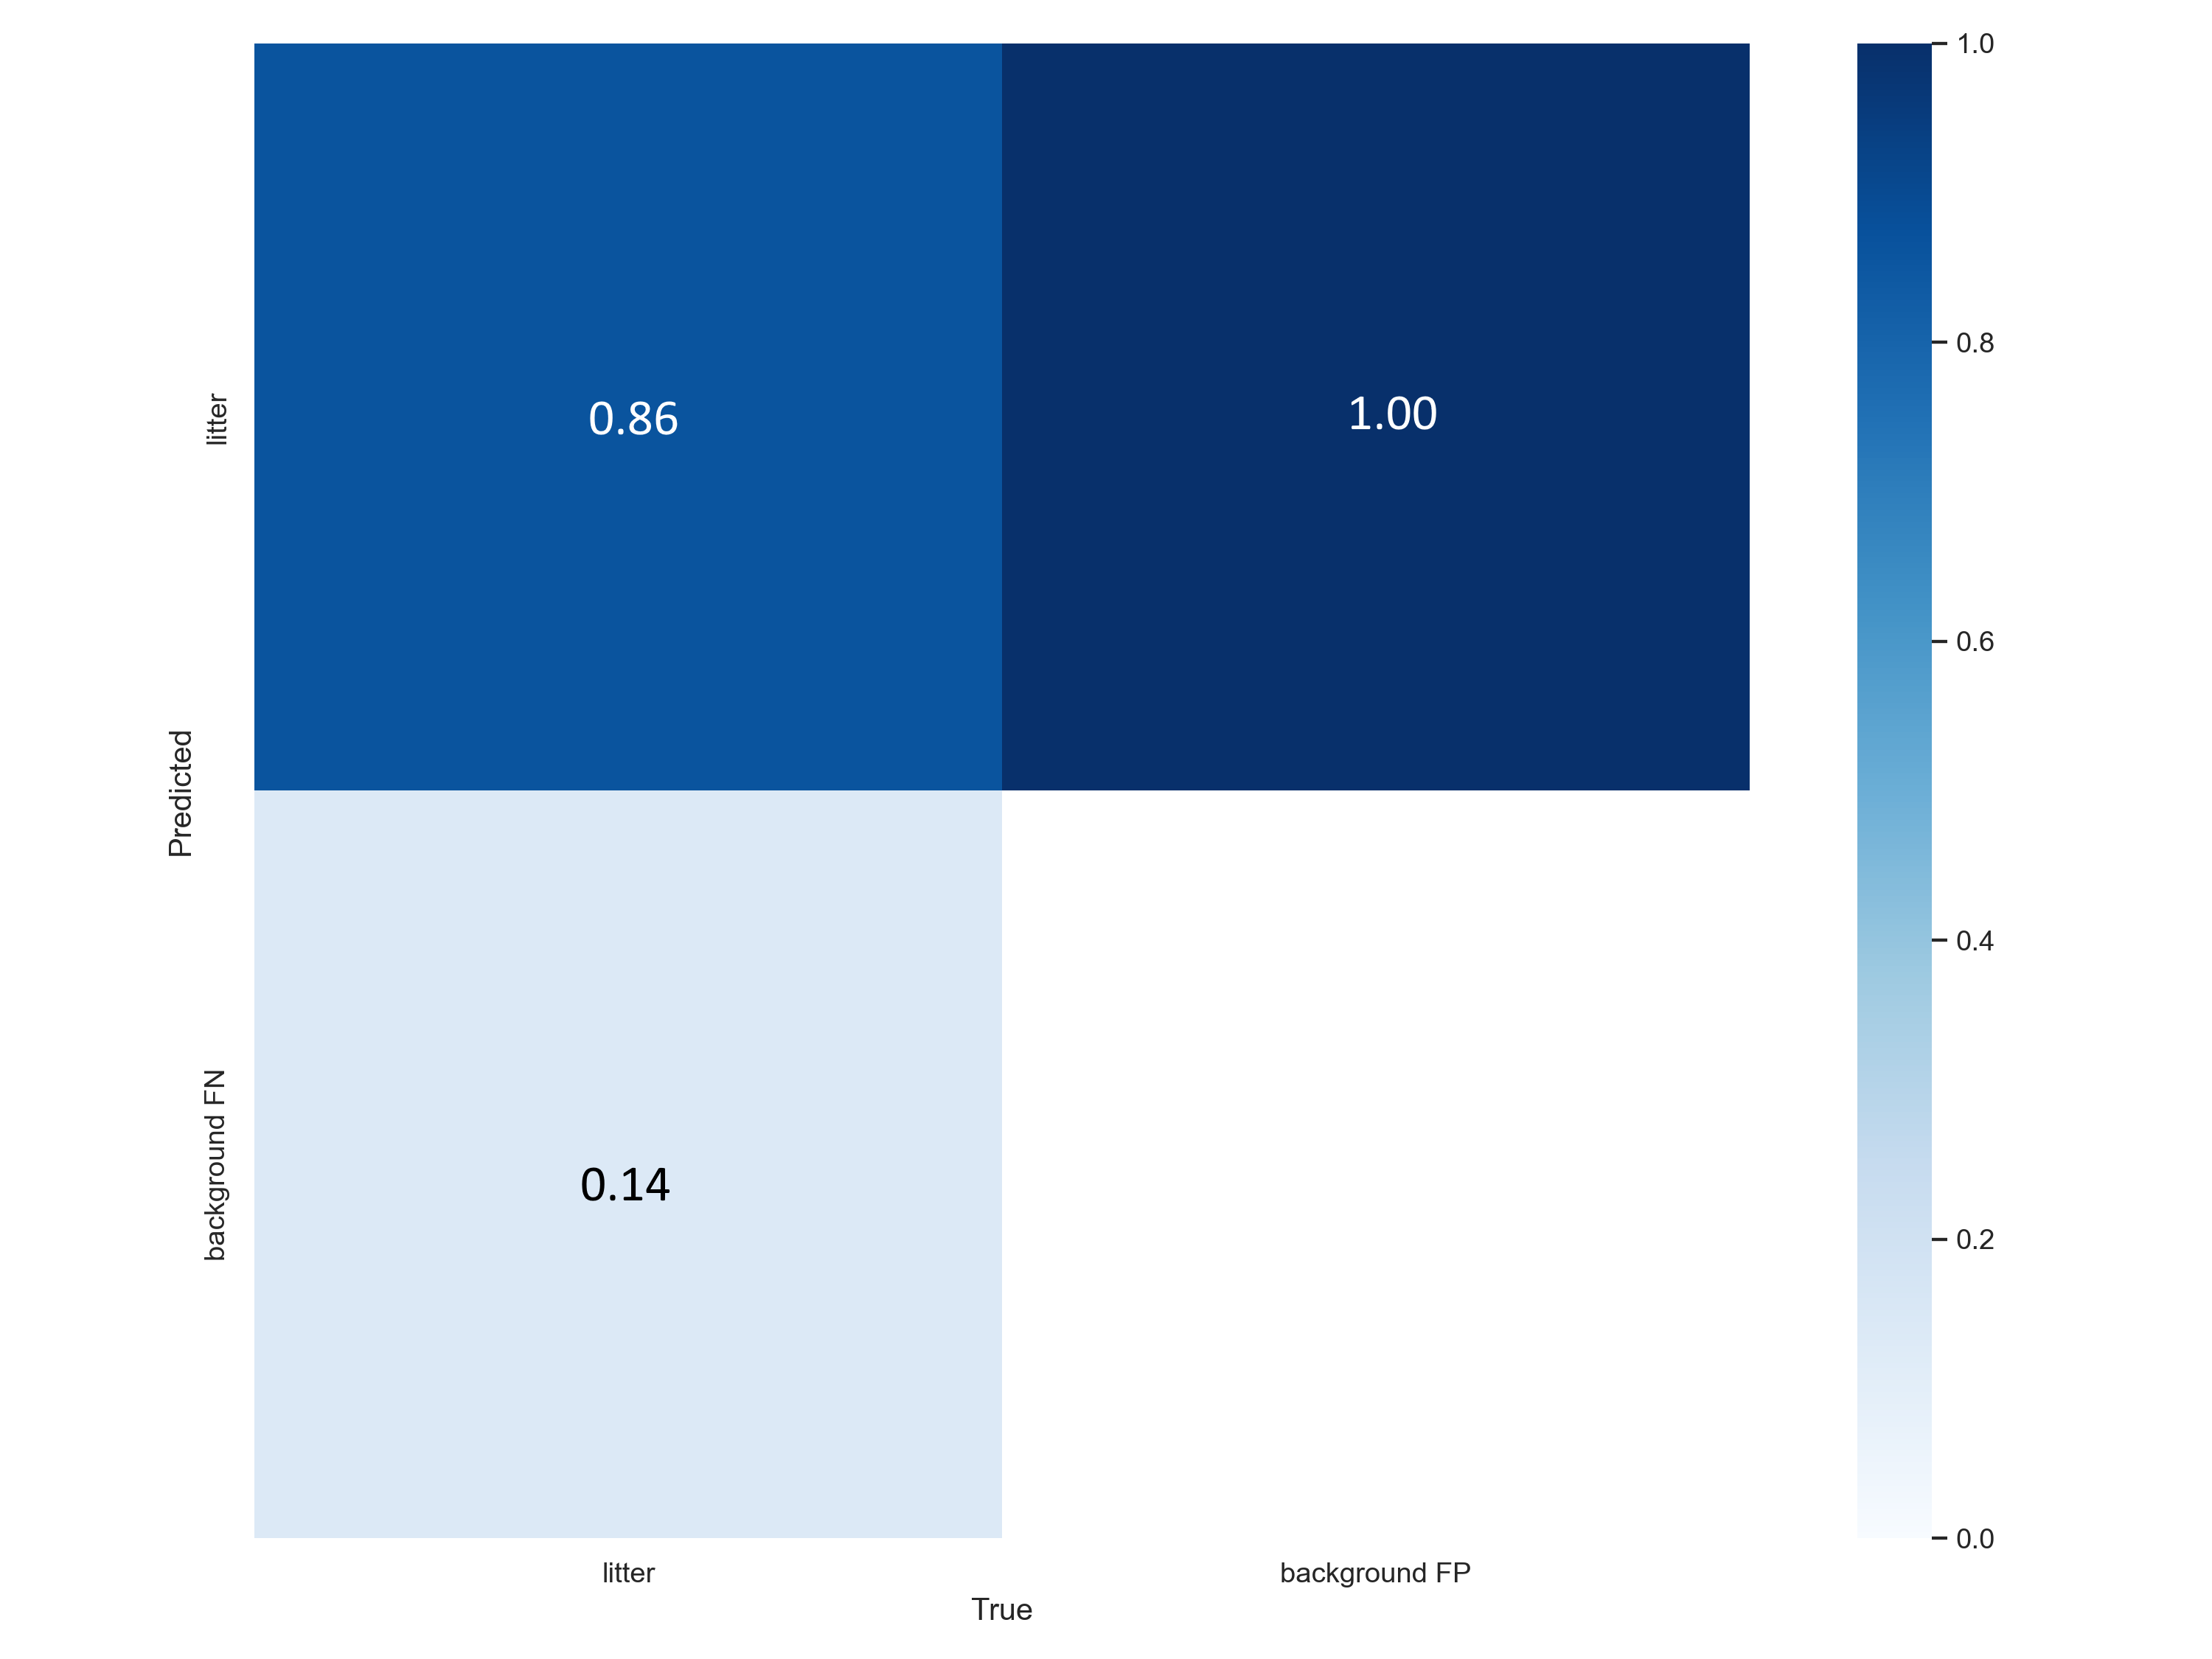
\includegraphics[scale=0.5]{images/fm-confusion-matrix.png}
    \caption{The confusion matrix of the litter detection model when applied to the test data. This shows a 77\% TPR, 23\% FNR, and tells us that every false positive was a member of the litter class.}
    \label{fig:fm-confusion-matrix}
\end{figure}

\end{appendices}

% Bibliography ================================================================

\newgeometry{bottom=1cm}
\bibliographystyle{unsrt}
\renewcommand{\thechapter}{0} % Don't number the bibliography
\bibliography{thesis}

\end{document}
